%%%%%%%%%%%%%%%%%%%%%%%%%%%%%%%%%%%%%%%%%%%%%%%%%%%%%%%%%%%%%%%%%%%%%%%%%%%%%%%%
%% Plantilla de memoria en LaTeX para la ETSIT - Universidad Rey Juan Carlos
%%
%% Por Gregorio Robles <grex arroba gsyc.urjc.es>
%%     Grupo de Sistemas y Comunicaciones
%%     Escuela Técnica Superior de Ingenieros de Telecomunicación
%%     Universidad Rey Juan Carlos
%% (muchas ideas tomadas de Internet, colegas del GSyC, antiguos alumnos...
%%  etc. Muchas gracias a todos)
%%
%% La última versión de esta plantilla está siempre disponible en:
%%     https://github.com/gregoriorobles/plantilla-memoria
%%
%% Para obtener PDF, ejecuta en la shell:
%%   make
%% (las imágenes deben ir en PNG o JPG)

%%%%%%%%%%%%%%%%%%%%%%%%%%%%%%%%%%%%%%%%%%%%%%%%%%%%%%%%%%%%%%%%%%%%%%%%%%%%%%%%

\documentclass[a4paper, 12pt]{book}
%\usepackage[T1]{fontenc}
\usepackage[utf8]{inputenc}
\usepackage[a4paper, left=2.5cm, right=2.5cm, top=3cm, bottom=3cm]{geometry}
\usepackage{times}
%\usepackage[latin1]{inputenc}
\usepackage[spanish]{babel} % Comenta esta línea si tu memoria es en inglés
\usepackage{url}
%\usepackage[dvipdfm]{graphicx}
\usepackage{graphicx}
\usepackage{float}  %% H para posicionar figuras
\usepackage[nottoc, notlot, notlof, notindex]{tocbibind} %% Opciones de índice
\usepackage{latexsym}  %% Logo LaTeX

\title{Análisis de proyectos Python de GitHub con Coala}
\author{Raúl Sánchez López}

\renewcommand{\baselinestretch}{1.5}  %% Interlineado

\begin{document}

\renewcommand{\refname}{Bibliografía}  %% Renombrando
\renewcommand{\appendixname}{Apéndice}

%%%%%%%%%%%%%%%%%%%%%%%%%%%%%%%%%%%%%%%%%%%%%%%%%%%%%%%%%%%%%%%%%%%%%%%%%%%%%%%%
% PORTADA

\begin{titlepage}
\begin{center}
\begin{tabular}[c]{c c}
%\includegraphics[bb=0 0 194 352, scale=0.25]{logo} &
\includegraphics[scale=0.25]{img/logo_vect.png} &
\begin{tabular}[b]{l}
\Huge
\textsf{UNIVERSIDAD} \\
\Huge
\textsf{REY JUAN CARLOS} \\
\end{tabular}
\\
\end{tabular}

\vspace{3cm}

\Large
INGENIERÍA DE TELECOMUNICACIÓN

\vspace{0.4cm}

\large
Curso Académico 2016/2017

\vspace{0.8cm}

Proyecto Fin de Carrera

\vspace{2.5cm}

\LARGE
ANÁLISIS DE PROYECTOS PYTHON DE GITHUB CON COALA

\vspace{4cm}

\large
Autor : Raúl Sánchez López \\
Tutor : Dr. Gregorio Robles
\end{center}
\end{titlepage}

\newpage
\mbox{}
\thispagestyle{empty} % para que no se numere esta pagina


%%%%%%%%%%%%%%%%%%%%%%%%%%%%%%%%%%%%%%%%%%%%%%%%%%%%%%%%%%%%%%%%%%%%%%%%%%%%%%%%
%%%% Para firmar
\clearpage
\pagenumbering{gobble}
\chapter*{}

\vspace{-4cm}
\begin{center}
\LARGE
\textbf{Proyecto Fin de Carrera}

\vspace{1cm}
\large
Análisis de proyectos Python de GitHub con Coala

\vspace{1cm}
\large
\textbf{Autor :} Raúl Sánchez López \\
\textbf{Tutor :} Dr. Gregorio Robles Martínez

\end{center}

\vspace{1cm}
La defensa del presente Proyecto Fin de Carrera se realizó el día \qquad$\;\,$ de \qquad\qquad\qquad\qquad \newline de 2017, siendo calificada por el siguiente tribunal:


\vspace{0.5cm}
\textbf{Presidente:}

\vspace{1.2cm}
\textbf{Secretario:}

\vspace{1.2cm}
\textbf{Vocal:}


\vspace{1.2cm}
y habiendo obtenido la siguiente calificación:

\vspace{1cm}
\textbf{Calificación:}


\vspace{1cm}
\begin{flushright}
Fuenlabrada, a \qquad$\;\,$ de \qquad\qquad\qquad\qquad de 2017
\end{flushright}

%%%%%%%%%%%%%%%%%%%%%%%%%%%%%%%%%%%%%%%%%%%%%%%%%%%%%%%%%%%%%%%%%%%%%%%%%%%%%%%%
%%%% Dedicatoria

\chapter*{}
\pagenumbering{Roman} % para comenzar la numeracion de paginas en numeros romanos
\begin{flushright}
\textit{Dedicado a \\
mi familia.}
\end{flushright}

%%%%%%%%%%%%%%%%%%%%%%%%%%%%%%%%%%%%%%%%%%%%%%%%%%%%%%%%%%%%%%%%%%%%%%%%%%%%%%%%
%%%% Agradecimientos

\chapter*{Agradecimientos}
%\addcontentsline{toc}{chapter}{Agradecimientos} % si queremos que aparezca en el índice
\markboth{AGRADECIMIENTOS}{AGRADECIMIENTOS} % encabezado 

¡Por fin llegó el día! Con la entrega de este proyecto doy por terminada esta etapa de mi vida. Ha sido un camino largo, muchas horas de estudio, días de biblioteca, alegrías y decepciones, pero todo esfuerzo tiene su recompensa. Al final de esta etapa no solo me llevo el título, también me llevo un trocito de todas esas personas con las que he compartido mis días y que han estado ahí para hacerlo todo más llevadero.

A Celia, por tu amistad y apoyo incondicional; a Carlos, por todos esos momentos compartidos dentro y fuera de la universidad; a Álvaro, por esos días en su casa agobiados con las prácticas y las discusiones futboleras; a Borja, por esos primeros días y todos los viajes camino a la universidad; a Joel, Pedro, César, Larraco, Victor, Sergio, Hugo, Alberto, y a todos los que me dejo, con quienes he compartido muchas horas de estudio, dudas, alegrías, confidencias y muchísimas risas.

A mi tutor, Gregorio, por su ayuda y consejo para la realización de este trabajo.

A mis amigos, que fueron un apoyo y una vía de escape en momentos de agobio.

Y por supuesto a mi familia, que siempre me ha apoyado en todos los sentidos. Vero, gracias por estar siempre. Abuelos, por vuestra forma de afrontar las adversidades y demostrarme que es posible superar cualquier cosa. Pero sobre todo a mis padres, por todo su apoyo y el enorme esfuerzo que han hecho para que yo pudiera conseguir este objetivo, todo esto es tan mío como vuestro.

¡Gracias por todo!

%%%%%%%%%%%%%%%%%%%%%%%%%%%%%%%%%%%%%%%%%%%%%%%%%%%%%%%%%%%%%%%%%%%%%%%%%%%%%%%%
%%%% Resumen

\chapter*{Resumen}
%\addcontentsline{toc}{chapter}{Resumen} % si queremos que aparezca en el índice
\markboth{RESUMEN}{RESUMEN} % encabezado

Este proyecto tiene como objetivo la creación de una aplicación web para el análisis de
proyectos de GitHub con Coala. Este análisis puede dar una idea acerca de la calidad de
los proyectos analizados, ya que a través de los diferentes `bears' con los que cuenta, es
capaz de detectar un gran número de problemas tanto en el código como en el proyecto en sí mismo
y mostrarlos de forma clara y ordenada.

El diseño está basado en el modelo cliente-servidor, de modo que aunque ambos puedan estar
alojados en la misma máquina, existe una separación que permite por un lado centrarse en la
lógica de la aplicación y por otro en la presentación de los resultados.

La aplicación web se ha desarrollado con Python, utilizando Django, y tecnologías como Coala, 
BootStrap, CSS, HTML, JSON y JavaScript. El proyecto está enfocado al análisis de proyectos 
Python alojados en GitHub, aunque con unos pequeños cambios podría ser utilizado para analizar 
código de cualquier otro de los muchos lenguajes de programación que soporta Coala.

Los datos obtenidos tras el análisis con Coala se almacenan en una base de datos que el usuario
puede consultar a través de la página de la aplicación y utilizar las diferentes funcionalidades.
%%%%%%%%%%%%%%%%%%%%%%%%%%%%%%%%%%%%%%%%%%%%%%%%%%%%%%%%%%%%%%%%%%%%%%%%%%%%%%%%
%%%% Resumen en inglés

\chapter*{Summary}
%\addcontentsline{toc}{chapter}{Summary} % si queremos que aparezca en el índice
\markboth{SUMMARY}{SUMMARY} % encabezado

This project aims to create an application web in order to analyse GitHub projects with Coala. The analysis can provide an idea about the quality of the analysed projects, since through the variety of their `bears' it is able to detect a large number of problems both in the code and in the project itself and show the results clearly and organized.

The design is based on the client-server model, so that both can be hosted in the same computer but there is a separation between the application logic and the presentation of the results.

The application web has been developed with Python, using the Django framework, and technologies as Coala, BootStrap, CSS, HTML, JSON and JavaScript. The project is focused on the analysis of Python projects hosted in Github, however, with a few changes, it could be used to analyse code of any other language supported by Coala.

The collected data after Coala analysis are stored in a database that can be consulted by the users through the application web and use the application funcionalities.

%%%%%%%%%%%%%%%%%%%%%%%%%%%%%%%%%%%%%%%%%%%%%%%%%%%%%%%%%%%%%%%%%%%%%%%%%%%%%%%%
%%%%%%%%%%%%%%%%%%%%%%%%%%%%%%%%%%%%%%%%%%%%%%%%%%%%%%%%%%%%%%%%%%%%%%%%%%%%%%%%
% ÍNDICES %
%%%%%%%%%%%%%%%%%%%%%%%%%%%%%%%%%%%%%%%%%%%%%%%%%%%%%%%%%%%%%%%%%%%%%%%%%%%%%%%%

% Las buenas noticias es que los índices se generan automáticamente.
% Lo único que tienes que hacer es elegir cuáles quieren que se generen,
% y comentar/descomentar esa instrucción de LaTeX.

%%%% Índice de contenidos
\tableofcontents 
%%%% Índice de figuras
\cleardoublepage
%\addcontentsline{toc}{chapter}{Lista de figuras} % para que aparezca en el indice de contenidos
\listoffigures % indice de figuras
%%%% Índice de tablas
%\cleardoublepage
%\addcontentsline{toc}{chapter}{Lista de tablas} % para que aparezca en el indice de contenidos
%\listoftables % indice de tablas


%%%%%%%%%%%%%%%%%%%%%%%%%%%%%%%%%%%%%%%%%%%%%%%%%%%%%%%%%%%%%%%%%%%%%%%%%%%%%%%%
%%%%%%%%%%%%%%%%%%%%%%%%%%%%%%%%%%%%%%%%%%%%%%%%%%%%%%%%%%%%%%%%%%%%%%%%%%%%%%%%
% INTRODUCCIÓN %
%%%%%%%%%%%%%%%%%%%%%%%%%%%%%%%%%%%%%%%%%%%%%%%%%%%%%%%%%%%%%%%%%%%%%%%%%%%%%%%%

\cleardoublepage
\chapter{Introducción}
\label{sec:intro} % etiqueta para poder referenciar luego en el texto con ~\ref{sec:intro}
\pagenumbering{arabic} % para empezar la numeración de página con números

\section{Presentación}
\label{sec:presentacion}
El presente documento es la memoria de el trabajo realizado para el proyecto fin de carrera de Ingeniería de Telecomunicación. El proyecto consiste en la creación de una herramienta para analizar proyectos Python alojados en la plataforma GitHub, apoyado en la herramienta Coala.

A la hora de desarrollar un proyecto es importante localizar y solventar los posibles problemas que se presenten. Si contamos con una herramienta que pueda detectar posibles errores y, adicionalmente, alertar sobre discrepancias con la guía de estilo del lenguaje de programación que estemos usando, tendremos la información necesaria para ayudarnos a solucionar los errores y mejorar la calidad de nuestro proyecto.

La aplicación web almacena la información recogida tras analizar los proyectos y la muestra de forma ordenada a varios niveles, facilitando la visualización de los datos. En este caso, la aplicación se ha orientado al análisis de proyectos Python, aunque puede servir como punto de partida para, haciendo algunos cambios, analizar proyectos desarrollados en otros lenguajes de programación, gracias a que Coala es compatible con un gran número de lenguajes de programación.

Básicamente contamos con dos funcionalidades principales: analizar proyectos y consultar los datos almacenados. A la hora de crear la interfaz web he pensado en la sencillez, de modo que el usuario pueda hacer uso de forma rápida, sencilla e intuitiva de las características de la herramienta, mostrando la información de forma clara y ordenada.

\section{Estructura de la memoria}
\label{sec:estructura}

La memoria está estructurada del siguiente modo:

\begin{itemize}
  \item \textbf{Capítulo 1. Introducción.} Descripción general del proyecto y breve explicación de la estructura del mismo.
  
  \item \textbf{Capítulo 2. Objetivos.} Exposición del objetivo general del trabajo, así como los objetivos más específicos que se pretenden alcanzar con este trabajo. Finalmente se incluye la planificación temporal seguida.
  
  \item \textbf{Capítulo 3. Estado del arte.} Descripción de las diferentes tecnologías utilizadas para el desarrollo de la aplicación web.
  
  \item \textbf{Capítulo 4. Diseño e implementación.} Explicación del desarrollo, estructura y funcionamiento del proyecto basado en las tecnologías descritas en el punto anterior.

  \item \textbf{Capítulo 5. Resultados.} Análisis de los resultados obtenidos.

  \item \textbf{Capítulo 6. Conclusiones.} Reflexión y conclusiones finales sobre el desarrollo del proyecto.
\end{itemize}



%%%%%%%%%%%%%%%%%%%%%%%%%%%%%%%%%%%%%%%%%%%%%%%%%%%%%%%%%%%%%%%%%%%%%%%%%%%%%%%%
%%%%%%%%%%%%%%%%%%%%%%%%%%%%%%%%%%%%%%%%%%%%%%%%%%%%%%%%%%%%%%%%%%%%%%%%%%%%%%%%
% OBJETIVOS %
%%%%%%%%%%%%%%%%%%%%%%%%%%%%%%%%%%%%%%%%%%%%%%%%%%%%%%%%%%%%%%%%%%%%%%%%%%%%%%%%

\cleardoublepage
\chapter{Objetivos}
\label{chap:objetivos}

\section{Objetivo general}
\label{sec:objetivo-general}
El objetivo principal de este trabajo es desarrollar una aplicación web que sirva a analizar el código fuente de proyectos Python y mostrar los resultados de estos análisis.

\section{Objetivos específicos}
\label{sec:objetivos-especificos}
Para alcanzar el objetivo principal se han perseguido los siguientes objetivos específicos:
\begin{itemize}
  \item Estudiar las funcionalidades de Coala y de los `bears' compatibles con Python.
  \item Examinar resultados de análisis con Coala a partir del fichero JSON generado y mapear estos datos para tratarlos posteriormente.
  \item Crear la primera versión de la herramienta capaz de analizar una lista de proyectos Python alojados en GitHub.
  \item Trasladar la herramienta a la aplicación web con Django, adaptando las vistas y organizando la base de datos para mostrar la información obtenida de forma sencilla.
  \item Optimizar el código y aplicación de mejoras visuales que faciliten el uso de la herramienta de forma que esta sea más rápida y sencilla de utilizar.
\end{itemize}


\section{Planificación temporal}
\label{sec:planificacion-temporal}
El presente proyecto surge a partir de otra idea inicial que si bien estaba relacionada, es un tanto distinta. La planificación temporal seguida para la elaboración de este proyecto, teniendo en cuenta que entre hitos he mantenido reuniones con mi tutor, ha sido la siguiente:

\begin{itemize}
  \item Reunión con el tutor en busca de ayuda y consejo para la elaboración del proyecto. En ella acordamos tomar como base Coala para analizar proyectos Python.
  \item Estudio de la herramienta Coala, para aprender como se usa, la diferentes funcionalidades, funcionamiento de los `bears' y ficheros de configuración,... Además del estudio de los resultados del análisis de Coala y los ficheros JSON generados dependiendo de la configuración utilizada.
  \item Definición de la estructura de la base de datos, mapeo de JSON obtenidos y creación de una primera versión de la herramienta, con una salida rudimentaria para mostrar los resultados.
  \item Desarrollo de la aplicación web con Django, llevando el programa principal a las vistas y la estructura de la base de datos a los modelos de Django.
  \item Mejora de aspecto de la web e inclusión de nuevas funcionalidades como la búsqueda por URL o fichero, búsqueda de resultados y presentación de datos.
  \item Optimización de la aplicación, incluyendo tablas de resumen con enlaces a los resultados para disminuir los tiempos de ejecución de los análisis.
  \item Elaboración de la memoria.
\end{itemize}


%%%%%%%%%%%%%%%%%%%%%%%%%%%%%%%%%%%%%%%%%%%%%%%%%%%%%%%%%%%%%%%%%%%%%%%%%%%%%%%%
%%%%%%%%%%%%%%%%%%%%%%%%%%%%%%%%%%%%%%%%%%%%%%%%%%%%%%%%%%%%%%%%%%%%%%%%%%%%%%%%
% ESTADO DEL ARTE %
%%%%%%%%%%%%%%%%%%%%%%%%%%%%%%%%%%%%%%%%%%%%%%%%%%%%%%%%%%%%%%%%%%%%%%%%%%%%%%%%

\cleardoublepage
\chapter{Estado del arte}
Para la realización de este proyecto me he apoyado en tecnologías ya existentes que serán presentadas en este capítulo, desde la herramienta de análisis con la que se procesa cada proyecto hasta las herramientas utilizadas para mostrar los resultados en la aplicación web.

\section{Coala} 
\label{sec:seccion1}
Coala es una herramienta que proporciona una interfaz unificada para encontrar y arreglar problemas en el código con un único fichero de configuración (coafile), independientemente del lenguaje de programación utilizado. La herramienta permite obtener los resultados del análisis en un fichero JSON fácilmente analizable, o personalizarlo acorde a las necesidades.~\cite{coala:_coala}

Coala dispone de un conjunto de plugins denominados `bears' compatibles con diferentes lenguajes de programación incluyendo Python, C/C++, JavaScript, CSS o Java entre otros, además de plugins compatibles con todos los lenguajes.

En el presente proyecto, se ha utilizado Coala para analizar proyectos Python, por lo que sólo se han utilizado `bears' compatibles con este lenguaje de programación. Una vez ejecutada la herramienta, se ha analizado el fichero JSON generado por Coala.

\subsection{coafile}
\label{sec:seccion1.1}
Fichero de configuración\footnote{\url{http://docs.coala.io/en/latest/Users/coafile.html}} de Coala. Se pueden utilizar hasta tres coafiles para configurar la herramienta:

\begin{itemize}
  \item Coafile por proyecto: Por convención este fichero es nombrado como `.coafile' y se aloja en  el directorio raíz del proyecto. Con esta convención, solo hay que ejecutar Coala desde el directorio raíz y la herramienta tomará la configuración del fichero.

Los ajustes definidos en este fichero de configuración anulan la configuración dada por el resto de ficheros de configuración y solo pueden ser anulados por aquellas opciones de configuración que introduzcamos por línea de comandos.

El fichero de configuración se puede dividir en secciones y puede contener los `bears' que vamos a utilizar y las opciones de configuración para cada uno de ellos. Hay que tener en cuenta que la mayor parte de las opciones de configuración de los `bears' son opcionales, por lo que sólo estaremos obligados a incluir aquellas que sean necesarias para realizar el análisis correctamente.
  \item Coafile por usuario: Este fichero, nombrado como `.coarc', se coloca en el `home' para establecer los ajustes por defecto del usuario. Estos ajustes serán tomados en cuenta para todos los proyectos que vayan a ser analizados por el usuario, y solo anulan los que sean especificados por el fichero de configuración del sistema.
  \item Coafile por sistema: Es el fichero de configuración de más baja prioridad. El denominado `default\_coafile' debe situarse en el directorio de instalación de Coala y es válido para todos los usuarios que utilicen Coala en el sistema.
\end{itemize}

\subsection{Bears}
\label{sec:seccion1.2}
Los bears\footnote{\url{https://coala.io/#!/languages}} son los plugins utilizados por Coala para análizar código. Actualmente cuenta con 78 bears que cubren un total de 54 lenguajes de programación, pero en este caso me centraré en aquellos compatibles con Python:

\subsubsection{BanditBear}
\label{sec:seccion1.2.1}
Con este bear se analiza el código Python en busca de los problemas de seguridad más comunes con la herramienta Bandit\footnote{\url{https://github.com/openstack/bandit}}. Bandit procesa cada uno de los ficheros, construye un AST\footnote{\url{https://docs.python.org/2/library/ast.html}}, ejecuta los plugins adecuados contra los nodos AST y genera un informe. La herramienta cuenta con una lista de test que se identifican mediante un ID.

\begin{itemize}
  \item Lenguajes: Python, Python 2, Python 3
  \item Configuración
    \begin{itemize}
          \item BANDIT\_SKIPPED\_TESTS: De manera opcional, podemos indicar en el fichero de configuración el ID de los test que no queramos ejecutar. Por defecto, este bear no ejecuta los plugin: B105  hardcoded\_password\_string, B106  hardcoded\_password\_funcarg, B107  hardcoded\_password\_default, B404  import\_subprocess,\\ B603  subprocess\_without\_shell\_equals\_true, B606  start\_process\_with\_no\_shell y B607  start\_process\_with\_partial\_path
    \end{itemize}
\end{itemize}

\subsubsection{FilenameBear}
\label{sec:seccion1.2.2}
Este bear se puede aplicar a cualquier lenguaje de programación. Comprueba que el nombre de los ficheros siguen una convención.

\begin{itemize}
  \item Lenguajes: Todos
  \item Configuración
    \begin{itemize}
          \item FILE\_NAMING\_CONVENTION: De manera opcional, se puede indicar una de las siguientes convenciones de nombrado: camel (thisIsCamelCase) - pascal (ThisIsPascalCase) - snake (this\_is\_snake\_case) - space (This Is Space Case). Por defecto, elige `snake'.
          \item IGNORE\_UPPERCASE\_FILENAMES: De manera opcional, se puede indicar si se quiere ignorar los nombres de fichero completamente en mayúsculas. Por defecto se ignoran.
    \end{itemize}
\end{itemize}

\subsubsection{InvalidLinkBear}
\label{sec:seccion1.2.3}
Busca enlaces en los ficheros y comprueba si son válidos. Considera válido el enlace si el servidor responde con un código 2xx. Este bear hará peticiones HEAD a todas las URL del fichero, por lo que es potencialmente peligroso si el código contiene URLs que no deben ser visitadas. Por ejemplo, si el fichero contiene una línea como la siguiente do\_not\_ever\_open = `https://api.acme.inc/delete-all-data', este bear la visitará, borrando todos los datos.

\begin{itemize}
  \item Lenguajes: Todos
  \item Configuración
    \begin{itemize}
          \item NETWORK\_TIMEOUT o TIMEOUT: Se trata de un dict\footnote{\url{https://docs.python.org/2/library/stdtypes.html#typesmapping}} mapeando URLs y tiempos de espera para cada enlace. Las URLs con el mismo host que las contenidas en el dict, esperarán el tiempo indicado. También puede contener un campo comodín con la clave ‘*’ para el resto de URLs. Es opcional y por defecto viene vacío.
          \item LINK\_IGNORE\_REGEX o IGNORE\_REGEX: Una expresión regular para identificar las URLs a ignorar. Es opcional y tiene un valor por defecto para URLs del tipo `example.com'.
          \item LINK\_IGNORE\_LIST: Lista de URLs a ignorar. Es opcional y por defecto está vacía.
          \item FOLLOW\_REDIRECTS: Si está en ‘True’ corrige los enlaces con errores, pero ignora las URLs que son muy diferentes a la URL original.  Es opcional y por defecto su estado es ‘False’.
    \end{itemize}
\end{itemize}

\subsubsection{MypyBear}
\label{sec:seccion1.2.4}
Comprueba la escritura estática usando la herramienta Mypy\footnote{\url{http://mypy.readthedocs.io/en/latest/basics.html}}. La herramienta chequea el código en busca de los errores de tipado mas comunes. Estas anotaciones referentes al tipo dentro del código no interfieren al ejecutar el programa al tratarse de un analizador estático.

Mypy puede comprobar que el código sigue las reglas básicas de anotaciones basadas en comentarios para Python 2 y Python 3 (utilizando PEP 484\footnote{\url{https://www.python.org/dev/peps/pep-0484/}}).

\begin{itemize}
  \item Lenguajes: Python, Python 2, Python 3
  \item Configuración
    \begin{itemize}
          \item LANGUAGE: Con `Python' o `Python 3', chequea código Python 3.x, mientras que la opción `Python 2' chequea código en Python 2.x. Es opcional y la opción por defecto es `Python 3'.
          \item ALLOW\_UNTYPED\_FUNCTIONS: Si su valor es `True', permite funciones sin anotaciones de tipo o con anotaciones de tipo incompletas. Por defecto el valor es `True'.
          \item STRICT\_OPTIONAL: Habilita chequeos estrictos relacionados con tipos opcionales, comprobando que no se intentan realizar operaciones no admitidas en valores `None' o que no se utilizan valores `None' cuando se espera un valor no opcional. Esta característica aún es experimental\footnote{\url{http://mypy-lang.blogspot.com.es/2016/07/mypy-043-released.html}}. Es opcional y por defecto su valor es `False'.
          \item PYTHON\_VERSION: Permite especificar la versión de Python concreta. Es opcional y por defecto su valor es `None'.
          \item CHECK\_UNTYPED\_FUNCTION\_BODIES: Permite no chequear el interior de las funciones que no tengan anotaciones de tipo. Es opcional y por defecto su valor es `False'.
          \item ALLOW\_UNTYPED\_CALLS: Permite la llamada a funciones sin anotaciones de tipo desde funciones tipadas. Es opcional y por defecto su valor es `True'.
    \end{itemize}
\end{itemize}

\subsubsection{PEP8Bear}
\label{sec:seccion1.2.5}
Detecta y corrige código que no cumpla con las normas de la guía de estilo para Python (PEP8\footnote{\url{https://www.python.org/dev/peps/pep-0008/}}). Este bear no modifica la funcionalidad del código de ninguna manera.

\begin{itemize}
  \item Lenguajes: Python, Python 2, Python 3
  \item Configuración
    \begin{itemize}
          \item MAX\_LINE\_LENGTH: Permite definir el número máximo de caracteres por línea. Es opcional y por defecto son 79.
          \item INDENT\_SIZE o TAB\_WIDTH: Permite definir el número de espacios para cada nivel de indentación. Es opcional y por defecto 4.
          \item PEP\_IGNORE: Lista de errores o advertencias a ignorar. Es opcional y por defecto aparece vacío.
          \item PEP\_SELECT: Lista de errores o advertencias para aplicar exclusivamente. Es opcional y por defecto aparece vacío.
          \item LOCAL\_PEP8\_CONFIG: Si está a `True', `autopep8'\footnote{\url{https://pypi.python.org/pypi/autopep8}} (usado para corregir el código para que cumpla con la guia de estilo) deberá usar un fichero de configuración indicado. Es opcional y por defecto su valor es `False'.
    \end{itemize}
\end{itemize}

\subsubsection{PyCommentedCodeBear}
\label{sec:seccion1.2.6}
Detecta código fuente comentado en Python. No tiene opciones de configuración.

\begin{itemize}
  \item Lenguajes: Python, Python 2, Python 3
\end{itemize}

\subsubsection{PycodestyleBear}
\label{sec:seccion1.2.7}
Analiza el código con la herramienta Pycodestyle\footnote{\url{https://pycodestyle.readthedocs.io/en/latest/}}, formalmente conocida como PEP8. Sirve para chequear que el código sigue las convenciones de estilo definidas para Python en PEP8.

Pycodestyle permite agregar nuevas normas de forma sencilla gracias a su estructura, su salida es parseable, es ligero y contiene una completa suite de pruebas. Actualmente consta de un completo listado\footnote{\url{https://pycodestyle.readthedocs.io/en/latest/intro.html#error-codes}} de códigos de error y advertencia. Hay que tener en cuenta que en la configuración por defecto, se ignoran los códigos E121, E123, E126, E133, E226, E241, E242, E704 y W503, ya que se corresponden con reglas que no están aceptadas de forma unánime y PEP8 no obliga a que sean cumplidas. El código E133 es mutuamente exclusivo con el código E123.

\begin{itemize}
  \item Lenguajes: Python, Python 2, Python 3
  \item Configuración
    \begin{itemize}
          \item MAX\_LINE\_LENGTH: Permite definir el número máximo de caracteres por línea. Es opcional y por defecto son 79.
          \item PYCODESTYLE\_IGNORE: Lista con los errores a ignorar de entre todos los códigos\footnote{\url{http://www.pydocstyle.org/en/latest/error_codes.html}}. Es opcional y por defecto está vacío.
          \item PYCODESTYLE\_SELECT: Lista con los errores a detectar de entre todos los códigos. Es opcional y por defecto está vacío.
    \end{itemize}
\end{itemize}

\subsubsection{PyFlakesBear}
\label{sec:seccion1.2.8}
Analiza las ficheros Python en busca de errores con la herramienta PyFlakesBear\footnote{\url{https://github.com/PyCQA/pyflakes}}, que puede detectar problemas de sintaxis, código sin uso y elementos indefinidos.

Es una herramienta que no tiene en cuenta el estilo. Es mas limitado que otras herramientas debido a que sólo examina el árbol de sintaxis de los archivos de forma individual, pero esta característica también lo hace más rápido. No tiene disponibles opciones de configuración con Coala.

\begin{itemize}
  \item Lenguajes: Python, Python 3
\end{itemize}

\subsubsection{PyImportSortBear}
\label{sec:seccion1.2.9}
Detecta los casos relacionados con la forma en que se ordenan los imports y es capaz de añadir comentarios basados en las muchas opciones de configuración que posee. Se basa en la herramienta `isort'\footnote{\url{https://isort.readthedocs.io/en/latest/}}, que se utiliza para ordenar los `imports' alfabéticamente y por secciones.

\begin{itemize}
  \item Lenguajes: Python, Python 2, Python 3
  \item Configuración
    \begin{itemize}
          \item USE\_PARENTHESES\_IN\_IMPORT:`True' si se utilizarán paréntesis en la declaración de los imports. Es opcional y por defecto es `True'.
          \item FORCE\_ALPHABETICAL\_SORT\_IN\_IMPORT: Si su valor es `True', fuerza a que todos los imports sean ordenados en una sola sección, en lugar de estar dentro de otros grupos. Es opcional y por defecto es `False'.
          \item FORCE\_SORT\_WITHIN\_IMPORT\_SECTIONS: Si su valor es `True', los imports estarán ordenados según su sección sin importar el tipo. Es opcional y por defecto es `True'.
          \item FROM\_FIRST\_IN\_IMPORT: Si es `True', los imports usando `from' se muestran encima del resto. Es opcional y por defecto es `False'.
          \item INCLUDE\_TRAILING\_COMMA\_IN\_IMPORT: Si es `True' añadirá una coma final a los imports. Ejemplo: `from abc import (a,b,c,)'. Es opcional y por defecto es `False'.
          \item COMBINE\_STAR\_IMPORTS: Si es `True', se asegura de que haya un `import *', y nada más es importado desde ese `namespace'. Es opcional y por defecto es `True'.
          \item COMBINE\_AS\_IMPORTS: Si es `True', isort combinará los imports dentro de la misma línea para las declaraciones de import. Es opcional y por defecto  es `True'.
          \item LINES\_AFTER\_IMPORTS: Fuerza que haya un cierto número de líneas después de la declaración de los imports y antes de la primera línea funcional de código. Por defecto es `-1', que utiliza 2 líneas si la primera línea de código es una clase o función y una línea para el resto de casos.
          \item ORDER\_IMPORTS\_BY\_TYPE: Si es `True', isort crea secciones separadas dentro de los `from' para constantes, clases y módulos/funciones. Es opcional y por defecto es `False'.
          \item BALANCED\_WRAPPING\_IN\_IMPORTS: Si es `True', para cada import multi-línea isort ajustará dinámicamente la longitud del import a una que guarde el equilibrio con la máxima longitud definida. Es opcional y por defecto es `False'.
          \item IMPORT\_HEADING\_LOCALFOLDER: Comentario colocado encima de los imports que comienza por `.'. Es opcional y por defecto está vacío.
          \item IMPORT\_HEADING\_FIRSTPARTY: Comentario colocado encima de los imports del proyecto. Es opcional y por defecto está vacío.
          \item IMPORT\_HEADING\_THIRDPARTY: Comentario colocado encima de los imports de terceros. Es opcional y por defecto está vacío.
          \item IMPORT\_HEADING\_STDLIB: Comentario colocado encima de los imports de la librería estándar. Es opcional y por defecto está vacío.
          \item IMPORT\_HEADING\_FUTURE: Comentario colocado encima de futuros imports. Es opcional y por defecto está vacío.
          \item DEFAULT\_IMPORT\_SECTION: Sección por defecto para colocar los imports si su sección no puede ser determinada automáticamente. Es opcional y por defecto es `FIRSTPARTY'.
          \item FORCE\_GRID\_WRAP\_IMPORTS: Fuerza a los `from' a estar dentro de la cuadrícula independientemente de la longitud de línea. Es opcional y por defecto es `False'.
          \item FORCE\_SINGLE\_LINE\_IMPORTS: Si es `True', cada import es forzado a mostrarse en una sola línea en lugar de tener imports multi-línea. Es opcional y por defecto es `True'.
          \item SORT\_IMPORTS\_BY\_LENGTH: Ordena los imports por longitud en lugar de alfabéticamente. Es opcional y por defecto es `False'.
          \item USE\_SPACES: Será `True' para utilizar espacios en lugar de tabulaciones. Es opcional y por defecto es `True'.
          \item INDENT\_SIZE: Número de espacios por nivel de indentación. Es opcional y por defecto es 4.
          \item FORCED\_SEPARATE\_IMPORTS: Lista de módulos que deseamos que aparezcan en una sección propia. Es opcional y por defecto está vacía.
          \item ISORT\_MULTI\_LINE\_OUTPUT\footnote{\url{https://isort.readthedocs.io/en/latest/#multi-line-output-modes}}: Entero que representa como se muestran los imports si no son lo suficientemente largos como para mostrarse en múltiples líneas. Es opcional y por defecto su valor es 4 (vert-grid).
          \item KNOWN\_FIRST\_PARTY\_IMPORTS: Lista de imports que está forzado a mostrar dentro de los imports del proyecto. Es opcional y por defecto está vacía.
          \item KNOWN\_THIRD\_PARTY\_IMPORTS: Lista de imports que está forzado a mostrar dentro de la categoría de imports de terceros. Es opcional y por defecto está vacía.
          \item KNOWN\_STANDARD\_LIBRARY\_IMPORTS: Lista de imports que está forzado a mostrar dentro de la categoría estándar de imports. Es opcional y por defecto está vacía.
          \item MAX\_LINE\_LENGTH: Máximo número de caracteres por línea. Es opcional y por defecto es 79.
          \item IMPORTS\_FORCED\_TO\_TOP: Fuerza a que la lista de imports aparezca encima de su respectiva sección. Es opcional y por defecto está vacía.
          \item TAB\_WIDTH: Número de espacios por nivel de indentación. Es opcional y por defecto es 4.
    \end{itemize}
\end{itemize}

\subsubsection{PyLintBear}
\label{sec:seccion1.2.10}
Chequea el código con PyLint\footnote{\url{https://www.pylint.org/}}, ejecutándolo para cada fichero por separado. PyLint detecta errores de sintaxis, código no usado, errores de formato, duplicidad y problemas de seguridad, gracias al amplio listado de chequeos\footnote{\url{http://pylint-messages.wikidot.com/all-messages}} que lleva a cabo.

La herramienta cuenta con un listado de errores\footnote{\url{http://pylint-messages.wikidot.com/all-codes}} que serán mostrados por Coala.

\begin{itemize}
  \item Lenguajes: Python, Python 2, Python 3
  \item Configuración
    \begin{itemize}
          \item PYLINT\_DISABLE: Inhabilita los mensajes, reportes, categoría o chequeos correspondientes a las IDs dadas. Es opcional y por defecto es una lista vacía.
          \item PYLINT\_ENABLE: Habilita los mensajes, reportes, categoría o chequeos correspondientes a las IDs dadas. Es opcional y por defecto es una lista vacía.
          \item PYLINT\_RCFILE: Especifica el RCFile\footnote{\url{https://en.wikipedia.org/wiki/RCFile}} para PyLint. Es opcional y por defecto está vacío.
          \item PYLINT\_CLI\_OPTIONS: Opciones por línea de comandos que se quieran pasar a PyLint. Es opcional y por defecto está vacío.
    \end{itemize}
\end{itemize}

\subsubsection{PyUnusedCodeBear}
\label{sec:seccion1.2.11}
Detecta código en desuso. Por defecto está limitado a declaraciones `pass' e imports innecesarios.

\begin{itemize}
  \item Lenguajes: Python, Python 2, Python 3
  \item Configuración
    \begin{itemize}
          \item REMOVE\_ALL\_UNUSED\_IMPORTS: Si es `True', elimina todos los imports que no se utilizan. Puede tener efectos secundarios. Es opcional y por defecto es `False'.
    \end{itemize}
\end{itemize}

\subsubsection{PyDocStyleBear}
\label{sec:seccion1.2.12}
Comprueba la semántica y convenciones relacionadas con los `docstrings'\footnote{\url{https://www.python.org/dev/peps/pep-0257}} de Python.

\begin{itemize}
  \item Lenguajes: Python, Python 2, Python 3
  \item Configuración
    \begin{itemize}
          \item PYDOCSTYLE\_SELECT: Lista que especifica los errores que se van a chequear. No puede usarse a la vez que `PYDOCSTYLE\_IGNORE'. Es opcional y por defecto está vacío.
          \item PYDOCSTYLE\_IGNORE: Lista que especifica los errores que se van a ignorar. No puede usarse a la vez que `PYDOCSTYLE\_SELECT'. Es opcional y por defecto está vacío.
    \end{itemize}
\end{itemize}

\subsubsection{PyromaBear}
\label{sec:seccion1.2.13}
Comprueba que se llevan a cabo buenas prácticas en lo referente al empaquetado utilizando Pyroma\footnote{\url{https://github.com/regebro/pyroma}}. La herramienta Pyroma está destinada a calificar como de bien cumple con las mejores prácticas un proyecto Python, así como un listado con los puntos que podrían ser mejorados.

Pyroma puede ayudar a diseñar un proyecto agradable y fácilmente utilizable, así como mejorar el software Python de terceros.

No cuenta con opciones de configuración en Coala.

\begin{itemize}
  \item Lenguajes: Python, Python 3
\end{itemize}

\subsubsection{RadonBear}
\label{sec:seccion1.2.14}
Radon sirve para calcular la complejidad de un fichero dado.

\begin{itemize}
  \item Lenguajes: Python, Python 2, Python 3
  \item Configuración
    \begin{itemize}
          \item RADON\_RANKS\_INFO: Categorías, dadas por Radon, para tratar la gravedad INFO. Es opcional y por defecto es una lista vacía.
          \item RADON\_RANKS\_NORMAL: Categorías, dadas por Radon, para tratar la gravedad NORMAL. Es opcional y por defecto es '('C', 'D')'.
          \item RADON\_RANKS\_MAJOR:Categorías, dadas por Radon, para tratar la gravedad MAJOR. Es opcional y por defecto es '('E', 'F')'.
    \end{itemize}
\end{itemize}

\subsubsection{VultureBear}
\label{sec:seccion1.2.15}
Chequea el código Python utilizando Vulture\footnote{\url{https://github.com/jendrikseipp/vulture}}. Esta herramienta busca en el código clases, funciones y variables que no son utilizadas, lo que ayuda a limpiar y encontrar errores en el código.

Aunque Vulture es una herramienta muy útil, hay que tener en cuenta una serie de consideraciones. Debido a la naturaleza dinámica de Python, los analizadores de código estáticos como Vulture probablemente pueden saltarse partes del código en desuso. Además, el código que solo es llamado implícitamente puede ser reportado como código no utilizado.

No cuenta con opciones de configuración en Coala.

\begin{itemize}
  \item Lenguajes: Python, Python 3
\end{itemize}

\subsubsection{coalaBear}
\label{sec:seccion1.2.16}
Comprueba que la ortografía de `coala' es correcta dentro del código. No cuenta con opciones de configuración.

\begin{itemize}
  \item Lenguajes: Todos
\end{itemize}

\subsubsection{SpaceConsistencyBear}
\label{sec:seccion1.2.17}
Comprueba y corrige el espaciado. Incluye el uso de tabulaciones en lugar de espacios, espacios en blanco a la izquierda o al final de la línea y las nuevas líneas de texto que falten al final del fichero.

\begin{itemize}
  \item Lenguajes: Todos
  \item Configuración
    \begin{itemize}
          \item ALLOW\_TRAILING\_WHITESPACE: Si es `True', se permiten espacios o tabulaciones después del último carácter que no sea un espacio en blanco en la línea antes del salto de línea. Es opcional y por defecto es `False'.
          \item INDENT\_SIZE: Número de espacios por nivel de indentación. Es opcional y por defecto es 4.
          \item ENFORCE\_NEWLINE\_AT\_EOF: Fuerza o no a que haya una nueva línea al final del fichero. Es opcional y por defecto es `True'.
          \item TAB\_WIDTH: Número de espacios por tabulación. Es opcional y por defecto es 4.
          \item USE\_SPACES: Si es `True', deben usarse espacios en lugar de tabulaciones. Es obligatorio.
    \end{itemize}
\end{itemize}

\section{Python} 
\label{sec:seccion2}
Python~\cite{python:_python} es un lenguaje de programación de código abierto optimizado para la calidad, productividad, portabilidad e integración creado a finales de los ochenta por Guido van Rossum~\cite{lutz:_programming_python}~\cite{beazley:_essential_reference}. Sus principales características son:

\begin{itemize}
  \item Lenguaje de alto nivel: automatiza la mayoría de las tareas a bajo nivel y hace hincapié en que su sintaxis sea sencilla, de forma que se adapta de forma adecuada a la capacidad cognitiva humana.
  \item Interpretado: de forma que solo necesita de un interprete para ser ejecutado directamente, sin necesidad de compilador.
  \item Multiparadigma: soporta más de un paradigma de programación, es decir, permite programar utilizando más de un estilo de programación (orientada a objetos, funcional, dinámica,...)
  \item Tipado dinámico: una variable puede tomar valores de distinto tipo en distinto momento. Los tipos se asignan en tiempo de ejecución y no es necesario declararlos con la variable.
\end{itemize}

Python ha sido utilizado en todo el proyecto debido a su facilidad de uso y su compatibilidad con DJANGO. Además, se trata de un lenguaje ampliamente utilizado y que cuenta con mucho material de apoyo.

\section{Django} 
\label{sec:seccion3}
Django~\cite{django:_django}~\cite{bennet:_django} es un entorno de trabajo de alto nivel diseñado para alentar un desarrollo rápido y limpio, dando prioridad a un diseño pragmático. Con este entorno de trabajo solo hay que preocuparse de desarrollar la aplicación, sin tener en cuenta las consideraciones generales del desarrollo de aplicaciones web. Es un entorno versátil, flexible, rápidamente escalable, gratuito y de código abierto.

Django está diseñado para ayudar a los desarrolladores a llevar sus aplicaciones desde el concepto hasta su terminación lo más rápido posible. Incluye docenas de extras que podemos utilizar para manejar las tareas más comunes del desarrollo web, tales como autenticación de usuarios o administración de contenidos entre otros.

Otro de los aspectos importantes de Django es la seguridad. Django ayuda a evitar errores de seguridad comunes como la inyección de SQL, cross-site scripting\footnote{\url{http://www.cgisecurity.com/xss-faq.html#whatis}}, etc... Su sistema de autenticación de usuarios proporciona una forma segura de administrar cuentas de usuario y contraseñas.

He utilizado Django para desarrollar la aplicación por su facilidad a la hora de crear las vistas y el interfaz web con en el que se interactúa con la aplicación. Adicionalmente, con Django se simplifica considerablemente el manejo de bases de datos, un aspecto muy importante de este proyecto.

\section{GitHub} 
\label{sec:seccion4}
GitHub\footnote{\url{https://github.com/}} es una plataforma donde se almacenan repositorios, utilizando el control de versiones Git. Una de sus principales características es el desarrollo colaborativo. 

Cada proyecto tiene su propia página web, la posibilidad de hacer ramificaciones (forks), control de versiones, wikis, gestión de errores y la posibilidad de que otros desarrolladores colaboren en el proyecto.

En la realización de este proyecto he utilizado la plataforma para obtener proyectos Python que analizar, clonados en local con Git, así como para almacenar tanto la aplicación como la memoria del proyecto. De este modo, ambos son públicos y están disponibles para su consulta o contribuciones de otros desarrolladores.

\section{Git} 
\label{sec:seccion5}
Git~\cite{git:_git} es un sistema de control de versiones que sirve para gestionar los cambios que sufre un proyecto durante su desarrollo. Una vez añadimos los elementos que debe gestionar, podemos hacer los cambios necesarios y estos quedarán registrados, manteniendo un registro histórico de las acciones que realicemos y contando con la posibilidad de volver a un estado anterior del proyecto.

Se trata de una de las principales herramientas de control de versiones. Se ha utilizado en la realización de este proyecto tanto para clonar los proyectos Python que analiza la herramienta, a partir de las URLs de los proyectos en GitHub, como para llevar el control del propio proyecto.

\section{HTML} 
\label{sec:seccion6}
HTML (HyperText Markup Language)\footnote{\url{https://www.w3.org/html/}} es el lenguaje de marcado estándar utilizado para la creación de páginas web y sus elementos forman los bloques de construcción de todas las páginas web.~\cite{robson:_html_css}

En el presente proyecto se ha utilizado para la creación de las diferentes páginas web que muestra Django y con las que interactúa el usuario para analizar o ver la información almacenada sobre los proyectos.

\section{BootStrap} 
\label{sec:seccion7}
BootStrap~\cite{bootstrap:_bootstrap} es un framework de código abierto desarrollado originalmente por diseñadores y desarrolladores de Twitter en 2010. Sirvió para el desarrollo de herramientas internas en la empresa durante más de un año, hasta que fue lanzado públicamente en 2011.

La herramienta consta de una colección de elementos personalizables y funciones para facilitar el diseño de páginas web. Hace uso de CSS, elementos HTML diseñados y mejorados con clases extensibles, un sistema avanzado de cuadrícula, componentes reutilizables como iconos o listas desplegables y JavaScript.

BootStrap se puede utilizar de diferentes formas, pero en este caso he descargado la versión precompilada, que permite hacer un uso rápido de ella con las fuentes que incluye, y la versión precompilada de su CSS y JavaScript. Además, he usado la plantilla `Bootstrap theme' para la creación de las diferentes páginas con las que cuenta el proyecto, añadiendo o eliminando los elementos necesarios para mostrar la información deseada.

\section{CSS} 
\label{sec:seccion8}
CSS (Cascading Style Sheets) permite definir la forma en la que se muestra un contenido, facilitando a los desarrolladores el control sobre el formato y estilo de los documentos.~\cite{robson:_html_css}

La principal característica de CSS es que permite separar el contenido de la presentación. Un desarrollador puede controlar el formato y estilo de muchas páginas al mismo tiempo, ya que todas las páginas reflejaran el aspecto marcado en el CSS.
    
En este proyecto se utiliza CSS como parte de BootStrap, haciendo uso de las clases definidas por esta herramienta para mejorar la presentación de la aplicación web.

\section{JavaScript} 
\label{sec:seccion9}
JavaScript\footnote{\url{https://developer.mozilla.org/es/docs/Web/JavaScript}} es un lenguaje ligero e interpretado. Está orientado a objetos, es un lenguaje script multi-paradigma, basado en prototipos, dinámico e imperativo. Puede decirse que es el lenguaje de programación de las webs, aunque también es utilizado en otros entornos.

JavaScript sirve para especificar el comportamiento de las páginas web, y forma parte de la `triada' de tecnologías básicas para el desarrollo web junto con HTML y CSS.~\cite{flanagan:_js}

En este proyecto se ha utilizado JavaScript para ocultar o mostrar parte del contenido de las páginas. A la hora de mostrar la información de un proyecto o fichero, o tras analizar una lista de ellos, se presenta toda la información del mismo y gracias a JavaScript podemos ocultar parte de los datos para poder tener una visión global.

\section{JSON} 
\label{sec:seccion10}
JSON\footnote{\url{http://www.json.org/}} (JavaScript Object Notation) es un formato de texto ligero para el intercambio de datos. Es sencillo de leer e interpretar para humanos y puede ser fácilmente generado e interpretado por máquinas. Además, es un formato de texto totalmente independiente del lenguaje de programación y está formado por estructuras universales que son soportadas por todos ellos, por lo que es el lenguaje ideal para el intercambio de datos.

JSON está constituido por dos estructuras: una colección de pares nombre/valor y una lista ordenada de valores.

En este proyecto se ha utilizado JSON como formato de salida de los análisis con Coala. Al tratarse de estructuras básica y fácilmente interpretables, es perfecto para su posterior análisis e inclusión de resultados en la base de datos una vez hecho el mapeo.

%%%%%%%%%%%%%%%%%%%%%%%%%%%%%%%%%%%%%%%%%%%%%%%%%%%%%%%%%%%%%%%%%%%%%%%%%%%%%%%%
%%%%%%%%%%%%%%%%%%%%%%%%%%%%%%%%%%%%%%%%%%%%%%%%%%%%%%%%%%%%%%%%%%%%%%%%%%%%%%%%
% DISEÑO E IMPLEMENTACIÓN %
%%%%%%%%%%%%%%%%%%%%%%%%%%%%%%%%%%%%%%%%%%%%%%%%%%%%%%%%%%%%%%%%%%%%%%%%%%%%%%%%

\cleardoublepage
\chapter{Diseño e implementación}

\section{Arquitectura general} 
\label{sec:seccion11}
La aplicación desarrollada está basada en el modelo cliente-servidor. En este modelo, cada una de las partes ejecuta acciones diferentes: el cliente realiza peticiones a la aplicación a través de la interfaz web; y el servidor atiende estas peticiones y da una respuesta al cliente. Además, hay que tener el cuenta que la mayoría de las peticiones, sino todas, conllevan el acceso a la base de datos, ya sea para almacenar o extraer información.

Aunque cliente y servidor pueden estar alojados en la misma máquina, existe una separación lógica entre ambas partes.

La aplicación dispone de las siguientes funcionalidades: análisis de proyectos dada una URL perteneciente a un proyecto alojado en GitHub, análisis de proyectos dado un fichero de texto que contenga URLs de proyectos alojados en GitHub, búsqueda de datos almacenados en la base de datos (proyectos, ficheros o bears encontrados), eliminación de proyectos de la base de datos, resúmenes de proyectos, ficheros y bears almacenados en la base de datos.

\begin{figure}[H]
  \centering
  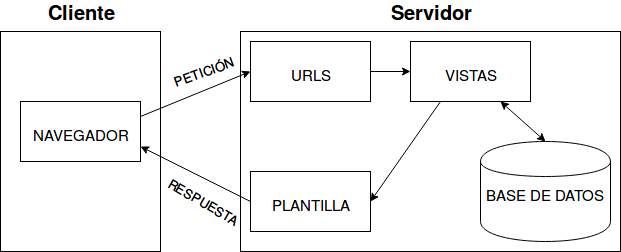
\includegraphics[width=9cm, keepaspectratio]{img/arqSistema}
  \caption{Esquema general de la aplicación.}
  \label{fig:arqSistema}
\end{figure}

\subsection{Servidor}
\label{sec:seccion11.1}
En el servidor es donde tenemos la aplicación en sí. Django dispone de un servidor por defecto, que es el que he utilizado para la realización de este proyecto.

A la hora de lanzar el servidor, Django permite elegir la IP y puerto en el que debe escuchar, pero se decidió utilizar la configuración por defecto: `localhost:8000', y todas las funcionalidades de la herramienta colgarán de `localhost:8000/analyzer/'.

Toda la lógica de la aplicación se encuentra en el fichero views.py. El cliente realiza una petición al servidor mediante la solicitud de una URL. La petición llega al controlador, que consulta en el fichero urls.py la vista asociada a esa URL y se hace la llamada a esa vista del fichero views.py. En este momento se ejecutan las acciones definidas en la vista y se consulta o actualiza la base de datos dependiendo de la acción concreta. Finalmente, se renderiza la página web a partir del template definido para cada caso y se envía al navegador mediante HTTP para que el cliente visualice el resultado de la consulta.


\subsection{Cliente}
\label{sec:seccion11.2}
En la parte del cliente es donde se encuentra el usuario de la aplicación, que accederá a ella a través de un navegador. El cliente realizará alguna de las peticiones descritas con anterioridad y las enviará al servidor. Una vez procesadas, recibirá la respuesta en forma de código HTML y será mostrada en el navegador.

Algunas templates utilizados en este proyecto cuentan con código JavaScript que permite esconder o mostrar parte de la información, por tanto el cliente también debe interpretar y ejecutar estos códigos.

\subsection{Base de datos}
\label{sec:seccion11.3}
La base de datos o el modelo como se conoce en Django, se define en el fichero models.py. Dentro del proyecto, la base de datos se organiza como muestra la figura~\ref{fig:EstructuraBBDD}.
\begin{figure}[H]
  \centering
  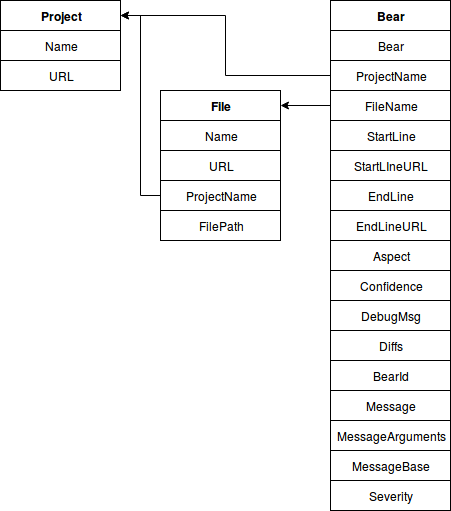
\includegraphics[width=9cm, keepaspectratio]{img/EstructuraBBDD}
  \caption{Estructura de la base de datos utilizada.}
  \label{fig:EstructuraBBDD}
\end{figure}
Se encuentra dentro del servidor y es consultada o actualizada por este en función de las peticiones del cliente. En ella se almacenan los datos obtenidos en los análisis de proyectos Python. Las distintas tablas se relacionan entre ellas por medio de los distintos campos, se trata de una base de datos relacional.

De este modo, cada Bear está asociado a un fichero y proyecto concreto; y cada fichero asociado a un proyecto tal y como se observa en la figura~\ref{fig:EstructuraBBDD}.

\section{Diseño e implementación del servidor} 
\label{sec:seccion12}
El servidor se encarga de procesar las peticiones y mostrar la información al cliente. Cada vez que el cliente hace una petición, el servidor hace las consultas necesarias a la base de datos, introduce los datos de los nuevos proyectos o actualiza los existentes.

\subsection{Análisis de proyectos}
\label{sec:seccion12.1}
Una de las principales características de la aplicación es el análisis de proyectos. Para hacer este análisis, existen dos posibilidades que el cliente puede elegir dentro de la página correspondiente: hacer el análisis de un solo proyecto a partir de la URL del proyecto alojado en GitHub o hacer un análisis masivo de proyectos desde un fichero de texto que contenga las URLs.

Cuando queremos analizar un solo fichero a partir de su URL, la aplicación se comporta según el diagrama de la figura~\ref{fig:AnalizarURL}.
\begin{figure}[H]
  \centering
  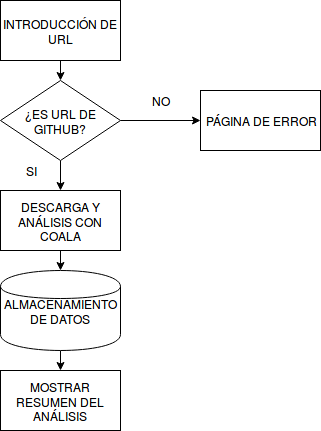
\includegraphics[width=7cm, keepaspectratio]{img/AnalizarURL}
  \caption{Diagrama de flujo en el análisis de proyectos por URL.}
  \label{fig:AnalizarURL}
\end{figure}
Cuando el cliente introduce una URL en el campo de texto, la aplicación comprueba se corresponde con una dirección de GitHub. Si la dirección no es correcta, se mostrará una página de error, y en caso contrario de clonará el proyecto con git en un directorio local. Si el proyecto ya existe en la base de datos, se sobrescribirá y se realizará el análisis sobre la última versión del proyecto.

Una vez descargado el proyecto, se analiza con Coala. Como solo vamos a analizar los ficheros Python, hay que ejecutar Coala sobre los ficheros con extensión `.py'. Además queremos que los resultados se muestren con la estructura de un JSON y redirigirlo a un fichero para su posterior análisis. Teniendo en cuenta todo esto, se ejecuta Coala del siguiente modo, utilizando un pipe:

{\footnotesize
\begin{verbatim}
    p1 = Popen(["coala", "--json", "--files", python_files], stdout=PIPE)
    p2 = Popen(["tee", settings.CONSTANTS['jsonFile']], stdin=p1.stdout, stdout=PIPE)
    p1.stdout.close()
    output = p2.communicate()[0]
\end{verbatim}
}

Donde `python\_files' son los ficheros con extensión `.py' y `settings.CONSTANTS[`jsonFile']' es la ruta definida en el fichero `settings' de Django para almacenar el fichero JSON con los datos del análisis. En este punto se elimina el proyecto del almacenamiento local, se lee el fichero JSON, se extraen los datos siguiendo el mapeo definido y se almacena todo en la base de datos\footnote{En la base de datos sólo se almacenan los ficheros analizados que contengan algún bear.}. Finalmente, se monta el código HTML sobre la plantilla y se envía para mostrar la información.

A continuación se muestra el aspecto del fichero JSON generado por Coala y desde donde se extraen los datos que se almacenan en la base de datos:

{\footnotesize
\begin{verbatim}
{
  "results": {
    "default": [
      {
        "additional_info": "",
        "affected_code": [
          {
            "end": {
              "column": null,
              "file": "/tmp/awesome-python/sort.py",
              "line": 14
            },
            "file": "/tmp/awesome-python/sort.py",
            "start": {
              "column": null,
              "file": "/tmp/awesome-python/sort.py",
              "line": 14
            }
          }
        ],
        "aspect": "NoneType",
        "confidence": 100,
        "debug_msg": "",
        "diffs": {
          "/tmp/awesome-python/sort.py": "--- \n+++ \n@@ -12,6 +12,7 @@\n     
            This could be extended by having nested blocks, sorting them 
            recursively\n and flattening the end structure into a list of 
            lines. Revision 2 maybe ^.^.\n \"\"\"\n+\n \n def sort_blocks
            ():\n     # First, we load the current README 
            into memory\n"
        },
        "id": 18970590811643698621472882157610514417,
        "message": "The code does not comply to PEP8.",
        "message_arguments": {},
        "message_base": "The code does not comply to PEP8.",
        "origin": "PEP8Bear",
        "severity": 1
      }
    ]
  }
}
\end{verbatim}
}

Cuando queremos analizar una lista de proyectos a partir de un fichero de texto, la aplicación se comporta según el diagrama de la figura~\ref{fig:AnalizarFichero}.

El fichero únicamente debe contener las URLs de GitHub correspondientes a los proyectos que se desee analizar y cada URL debe ir en una línea distinta.

Cuando el cliente introduce la ruta del fichero que contiene las URLs, el servidor comprueba que la ruta es válida y en caso contrario muestra una página de error. Una vez comprobado, el servidor lee el fichero línea a línea y sigue el mismo proceso que en el apartado anterior, que recordemos es: comprobar que la URL pertenece a un proyecto de GitHub, descarga del proyecto, análisis y almacenamiento de datos. Si alguno de los proyectos no puede ser analizado, la aplicación pasa a la siguiente línea.

Una vez terminado el análisis, se cargan los datos en el template correspondiente y se envía el código HTML al cliente para mostrar un resumen de todos los proyectos analizados. Para mostrar este resumen, cada vez que analizamos un proyecto se incluye en una lista y al finalizar se muestran los datos almacenados para los proyectos de esa lista.

\begin{figure}[H]
  \centering
  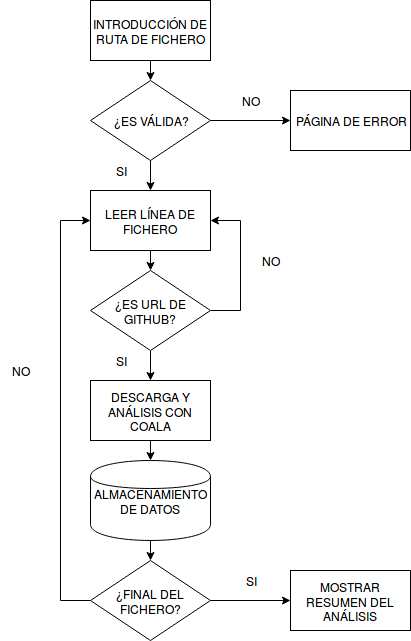
\includegraphics[width=7cm, keepaspectratio]{img/AnalizarFichero}
  \caption{Diagrama de flujo en el análisis de proyectos por fichero.}
  \label{fig:AnalizarFichero}
\end{figure}

\subsection{Búsqueda en la base de datos}
\label{sec:seccion12.2}
La aplicación permite hacer una búsqueda en la base de datos. Dentro de la sección correspondiente, el cliente debe elegir la categoría en la que quiere buscar: proyecto, fichero o bear. Una vez relleno el campo de texto y seleccionada la categoría, se lanza la búsqueda en el servidor.

El servidor recibe la consulta y la opción de búsqueda deseada y muestra todos los registros de la base de datos que encajan con la búsqueda junto con un pequeño resumen y links hacia la información al completo. En caso de no encontrar nada, mostrará un mensaje informando de la situación.

Hay que tener en cuenta que dependiendo de los criterios de búsqueda la operación tardará más o menos tiempo. La cantidad de bears almacenados suele ser muchísimo mayor que el número de ficheros y proyectos por lo que puede llevar bastante tiempo en comparación con otras búsquedas.

\subsection{Resumen de proyectos, ficheros y bears almacenados}
\label{sec:seccion12.3}
Otra de las funcionalidades de la aplicación es mostrar un resumen de todos los datos almacenados en la base de datos.

\subsubsection{Resumen de proyectos almacenados}
\label{sec:section12.3.1}
Cuando el cliente envía una petición para mostrar los datos de proyectos, el servidor recorre la lista de ficheros almacenados y cuenta todos los pertenecientes a ese proyecto. Repite la operación con los bears almacenados para contar la cantidad de bears encontrados. Finalmente, monta una tabla con estos datos, el enlace a la página que contiene todos los detalles del proyecto y el porcentaje de ficheros afectados respecto al número total de ficheros del proyecto antes de enviar el código HTML al cliente.

\subsubsection{Resumen de ficheros almacenados}
\label{sec:section12.3.2}
Cuando la petición del cliente es para mostrar los datos de los ficheros afectados por algún bear, el servidor recorre la lista de bears almacenados y cuenta todos aquellos que pertenecen a cada fichero, mostrando los bears totales por fichero. Finalmente monta una tabla de resumen con estos datos, el nombre el proyecto y enlaces a las páginas de detalle del fichero y proyecto al que pertenecen, y envía el código HTML al cliente.

\subsubsection{Resumen de bears almacenados}
\label{sec:section12.3.3}
Por último, cuando la consulta es acerca de los bears almacenados, el servidor recorre la lista de bears y anota el tipo de bear de cada uno. Al terminar, muestra todos los tipos de bear almacenados en la base de datos y la cantidad de cada uno de ellos, y envía el código HTML al cliente. 

En esta lista pueden aparecer repetidos algunos bears con un código al final, esto ocurre porque algunos bears se corresponden con herramientas que analizan diferentes aspectos del código. Por tanto, aunque el bear sea el mismo, el código hace referencia al aspecto concreto que se ha analizado en cada caso.

\subsection{Detalles de proyectos, ficheros y bears almacenados}
\label{sec:seccion12.4}
El cliente puede hacer una búsqueda para encontrar la información detallada de un proyecto, fichero o bear concreto, o acceder a los datos a través de alguno de los enlaces que aparecen en las diferentes páginas.

\subsubsection{Detalle de proyecto}
\label{sec:section12.4.1}
El cliente envía una petición al servidor cuando accede a la página de un proyecto a través de una URL del siguiente tipo:

{\footnotesize
\begin{verbatim}
    http://localhost:8000/analyzer/project/CREADOR_PROYECTO/NOMBRE_PROYECTO
\end{verbatim}
}

Al acceder a la página de información de un proyecto, el servidor busca el proyecto en la base de datos y en caso de que no exista la respuesta del servidor se mostrará en una página de error. Si el proyecto existe, muestra todos los campos almacenados, el número total de ficheros afectados y el porcentaje de ficheros afectados respecto al total de ficheros Python del proyecto. Además, recorre la lista de los ficheros relacionados con este proyecto y muestra un resumen del tipo y cantidad de bears encontrados para cada uno.

La información de los ficheros analizados está oculta por defecto y puede mostrarse si el usuario lo desea gracias al código JavaScript que contiene la página. Esto se hace para no amontonar la información en pantalla, de forma que el usuario vea un resumen de los datos y se muestre el resto si así lo desea.

\subsubsection{Detalle de fichero}
\label{sec:section12.4.2}
El cliente envía una petición al servidor cuando accede a la página de un fichero a través de una URL del siguiente tipo:

{\footnotesize
\begin{verbatim}
    http://localhost:8000/analyzer/file/CREADOR_PROY/NOMBRE_PROY/FICHERO
\end{verbatim}
}

Al acceder a la página de información de un proyecto, comprueba que existan en la base de datos tanto el proyecto como el fichero en cuestión. Si no existen se mostrará una página de error y en caso contrario se saca toda la información del fichero (nombre, proyecto al que pertenece, URL en GitHub y path local del fichero). Además, se recorren los bears asociados a este fichero y se extrae parte de la información como el nombre del bear, la línea del fichero donde se encontró, el mensaje del bear y su Id.

Como en el caso anterior, la información de bears encontrados se encuentra oculta por defecto y puede desplegarse gracias al código JavaScript insertado en el código HTML.

\subsubsection{Detalle de bear}
\label{sec:section12.4.3}
El cliente envía una petición al servidor cuando accede a la página de un bear a través de una URL del siguiente tipo:

{\footnotesize
\begin{verbatim}
    http://localhost:8000/analyzer/bear/ID_BEAR
\end{verbatim}
}

Cada ID es único, por tanto se comprueba que el bear correspondiente a esa Id se encuentra almacenado en la base de datos y en caso contrario se muestra una página de error. Si el bear existe en la base de datos, se extrae toda la información\footnote{Aspect, MessageArguments y MessageBase no se muestran por no aportar información extra al usuario.} y se monta el código HTML para en viarlo al cliente. Cada bear se corresponde con un proyecto y fichero concreto.

\subsection{Eliminación de proyectos almacenados}
\label{sec:seccion12.5}
Esta funcionalidad no aparece en la barra de navegación del cliente ya que está pensada para que el administrador pueda eliminar proyectos de la base de datos. Es posible que ocurra un error durante el análisis que deje datos incompletos del proyecto y por tanto es útil contar con la función de borrado a través de una URL construida de la siguiente forma:

{\footnotesize
\begin{verbatim}
    http://localhost:8000/analyzer/remove/CREADOR_PROYECTO/NOMBRE_PROYECTO
\end{verbatim}
}

\section{Diseño e implementación del cliente} 
\label{sec:seccion13}
Las peticiones al servidor se realizan a través de la parte del cliente, además el cliente se encarga de mostrar al usuario los resultados de esas consultas después de interpretar el código HTML recibido.

Gracias a Django, es posible hacer una separación entre la presentación final de la aplicación y la lógica de la misma. Para ello, he definido una serie de templates que servirán de base para el código HTML que se va a mostrar en cada caso. En el fichero `views.py' añadiremos la información en contexto dentro del template una vez procesada la petición del cliente para mostrar la respuesta.

Para la creación de estos templates, me he ayudado de BootStrap, que permite crear sitios web atractivos a la vista y con algunas funcionalidades realmente útiles. Además, gracias a BootStrap, el diseño de la aplicación se adapta al tamaño del dispositivo permitiendo una correcta visualización en cada caso, es decir, es un diseño `responsive'. Además, todas las páginas diseñadas cuentan con una barra de navegación superior que facilita el acceso a las diferentes funcionalidades que tiene la aplicación.

\begin{figure}[H]
  \centering
  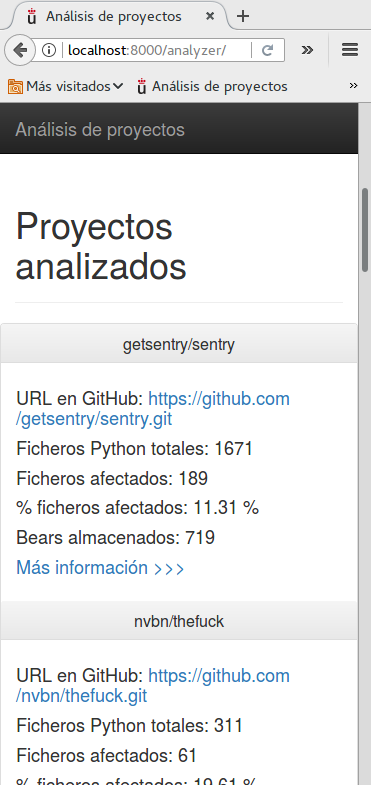
\includegraphics[width=4cm, keepaspectratio]{img/webAdaptativa}
  \caption{Página principal adaptada a una ventana pequeña.}
  \label{fig:webAdaptativa}
\end{figure}

La página principal muestra una breve explicación el proyecto y acto seguido una lista con todos los proyectos analizados ordenados en orden ascendente por el porcentaje de ficheros afectados por algún bear. Aunque la cantidad de bears encontrados depende en gran medida del tamaño del proyecto y los ficheros analizados, con un primer vistazo ya podemos ver un resumen de lo que nos encontraremos.

El usuario puede pinchar en `Más información' para acceder a la página de un proyecto dentro de la aplicación, o en el enlace de GitHub para inspeccionar el proyecto en la plataforma.

\begin{figure}[H]
  \centering
  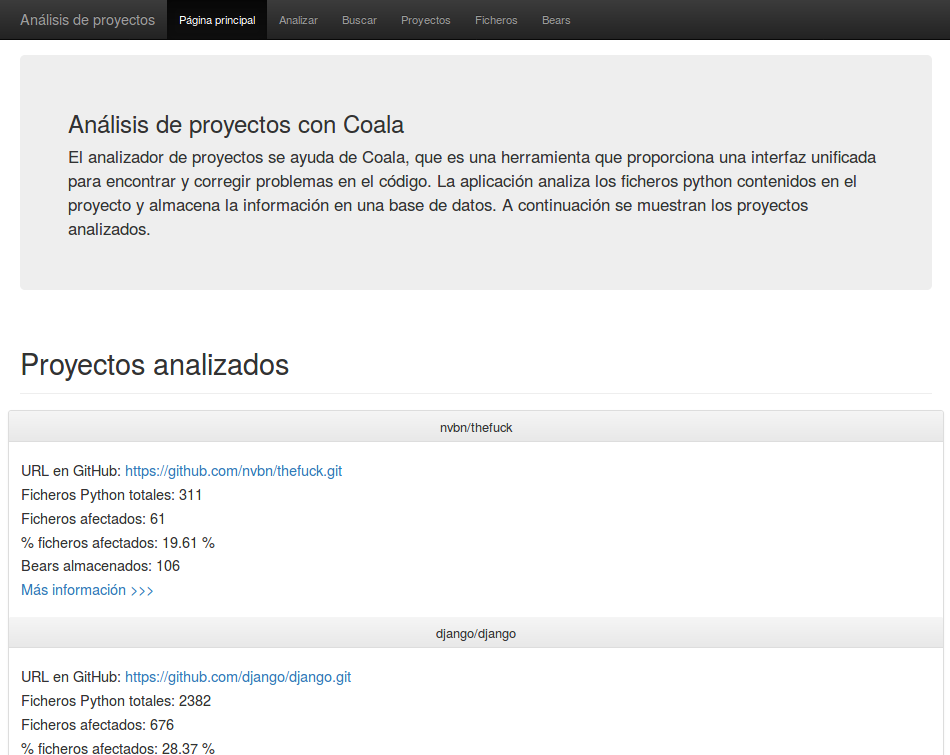
\includegraphics[width=16cm, keepaspectratio]{img/homePage}
  \caption{Página principal de la aplicación web.}
  \label{fig:homePage}
\end{figure}

Si el usuario quiere analizar un proyecto, o varios, al entrar en el apartado de análisis encontrará las dos posibles opciones: analizar a partir de una URL o analizar a partir de un fichero de texto. Al pulsar en la opción deseada, se mostrará la página correspondiente en la que el usuario debe introducir la URL o la ruta absoluta del fichero que contiene las URLs que se van a analizar.

Al concluir el análisis, en ambos casos se muestra un resumen de los proyectos analizados. En este resumen se incluye la información del proyecto y un resumen de ficheros y bears encontrados que podemos mostrar u ocultar pinchando en `Mostrar/ocultar ficheros analizados'. Si queremos ver los bears de cada tipo, al pinchar en el enlace haremos una búsqueda en la base de datos de ese tipo de bear o también podemos acceder a la página de información para el proyecto o alguno de los ficheros.

\begin{figure}[H]
  \centering
  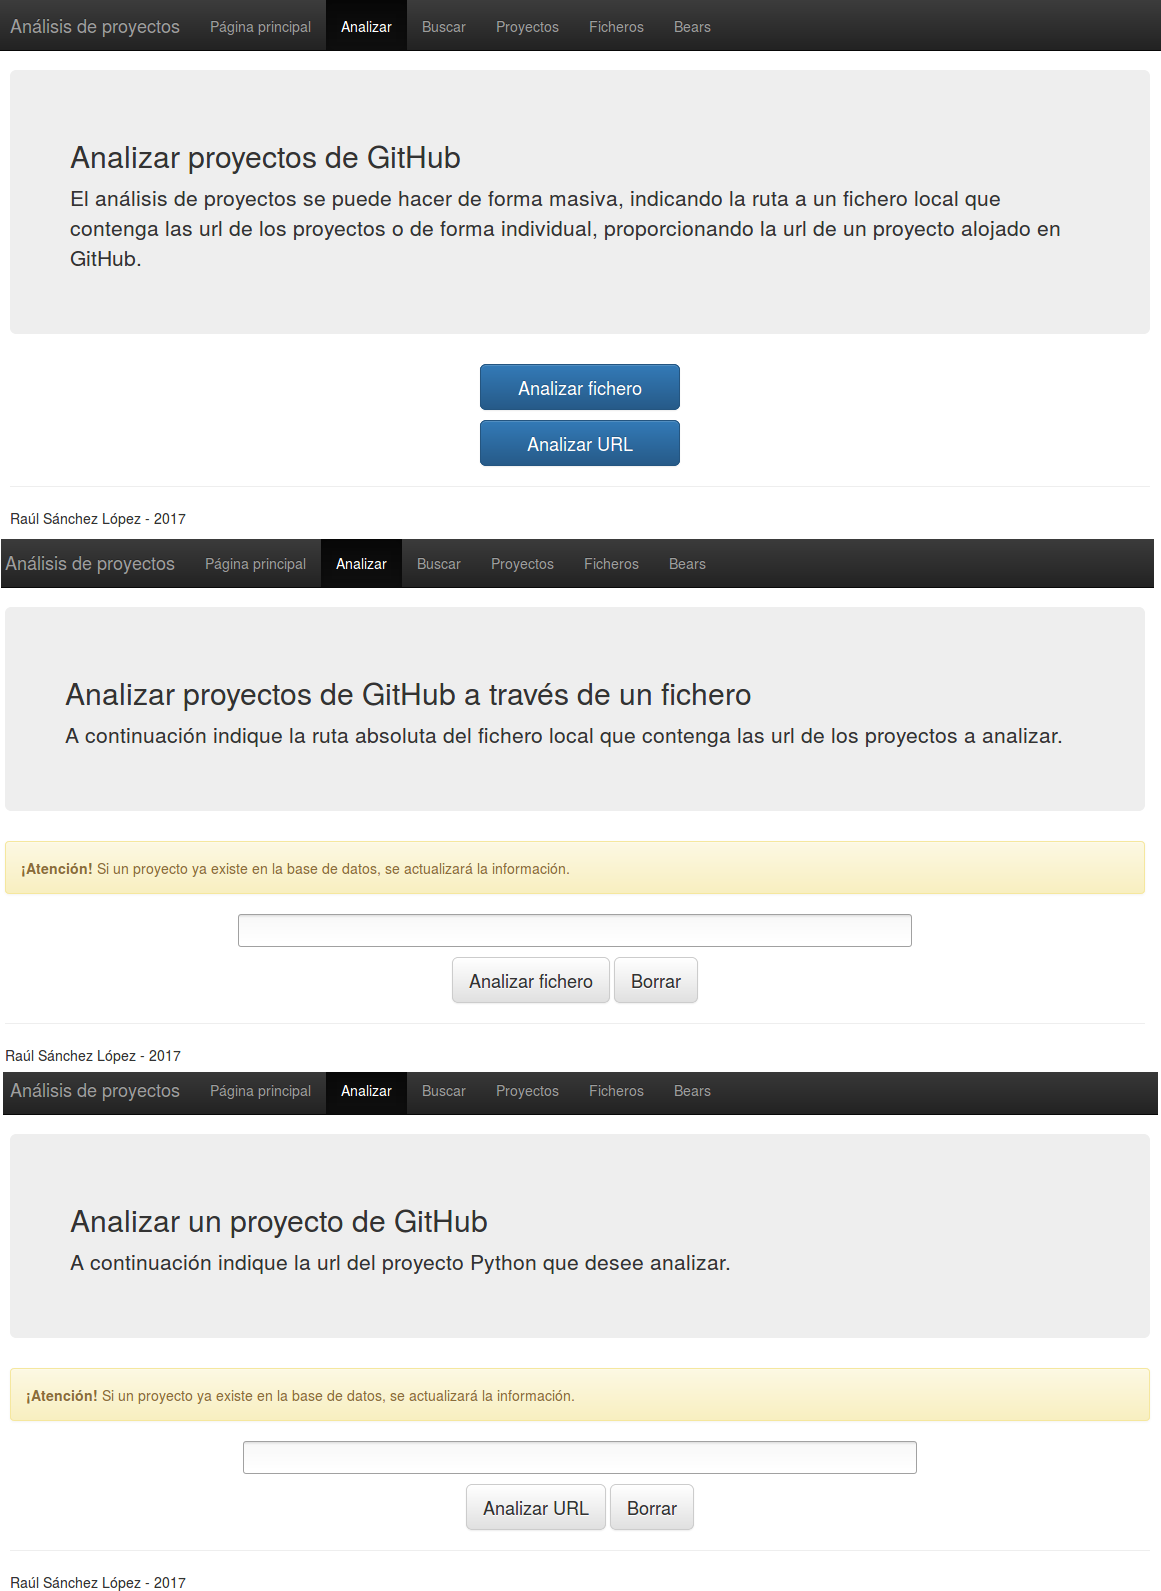
\includegraphics[width=15cm, keepaspectratio]{img/webAnalisis}
  \caption{Páginas de análisis. Arriba, la página principal; en el medio, la página de análisis a partir de un fichero; y abajo, la página de análisis a partir de una URL.}
  \label{fig:webAnalisis}
\end{figure}

\begin{figure}[H]
  \centering
  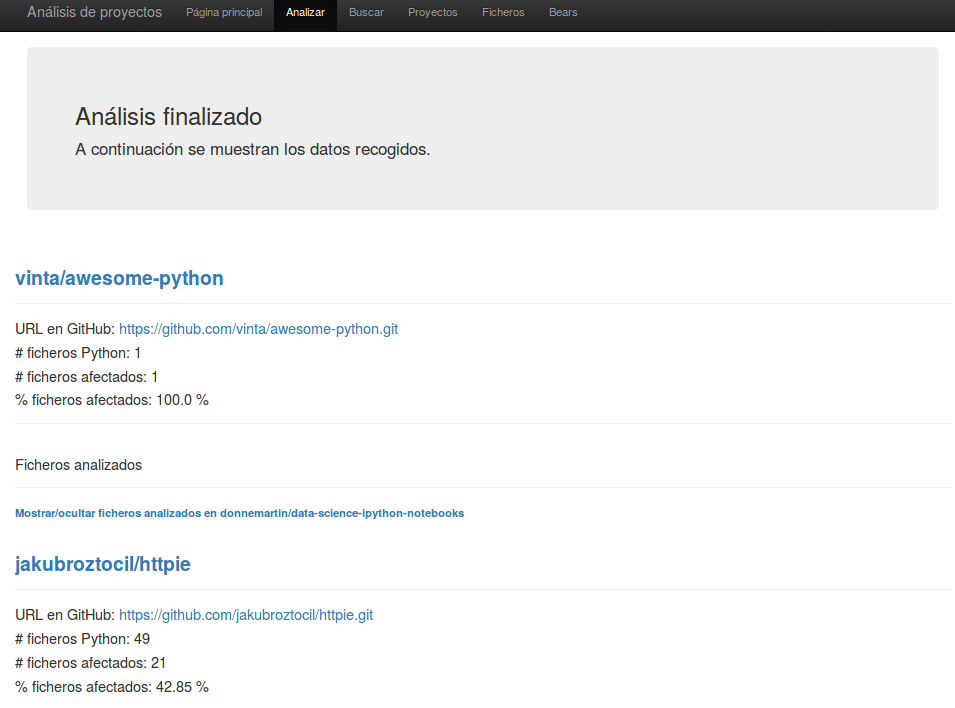
\includegraphics[width=12cm, keepaspectratio]{img/resumenAnalisis}
  \caption{Resumen del análisis realizado.}
  \label{fig:resumenAnalisis}
\end{figure}

La siguiente funcionalidad es la de buscar en la base de datos. Al acceder a esta página, nos muestra un cuadro de texto y las opciones entre las que podemos elegir para iniciar la búsqueda.

\begin{figure}[H]
  \centering
  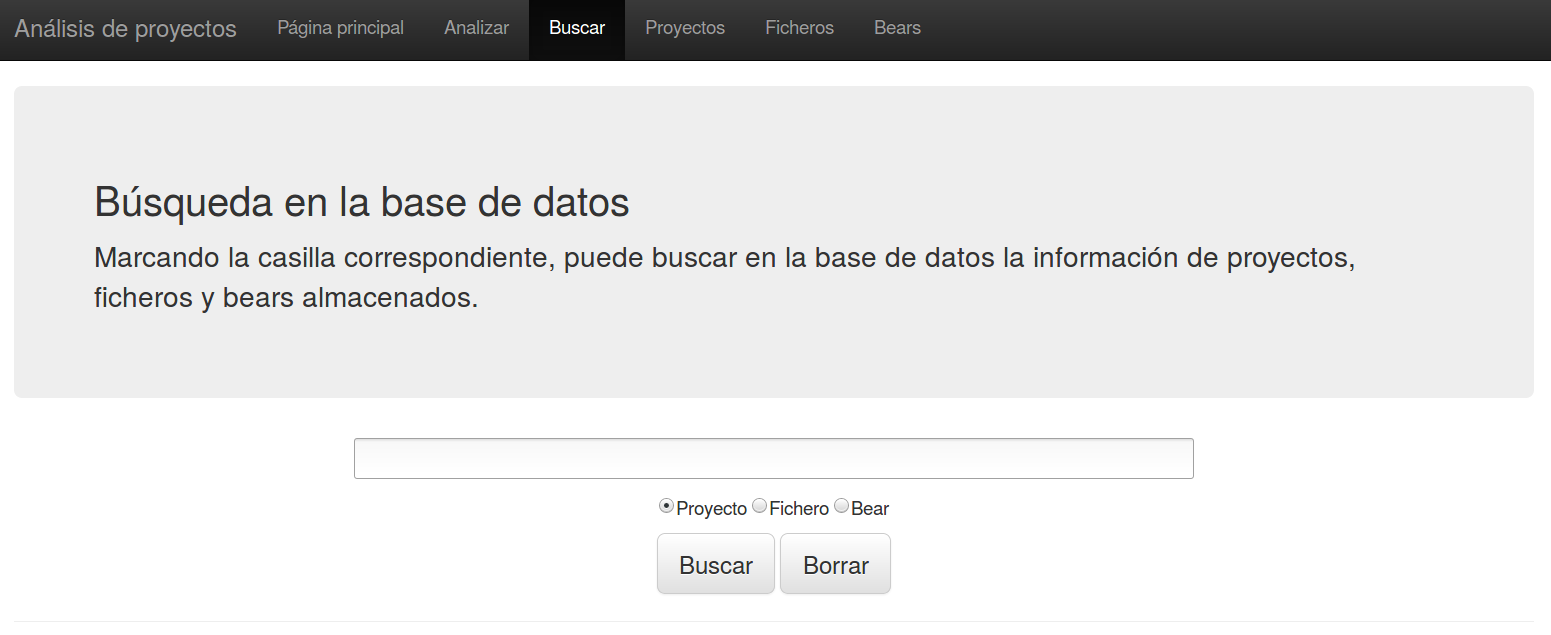
\includegraphics[width=15cm, keepaspectratio]{img/webBuscar}
  \caption{Página de búsqueda.}
  \label{fig:webBuscar}
\end{figure}

Una vez terminada, se muestra un listado con todos los datos encontrados. Si por ejemplo queremos buscar el fichero `sort.py', nos mostrará todos los ficheros con ese nombre almacenados, en este caso solo hay uno. En caso de que el fichero no se encuentre en la base de datos, mostrará un mensaje de error.

\begin{figure}[H]
  \centering
  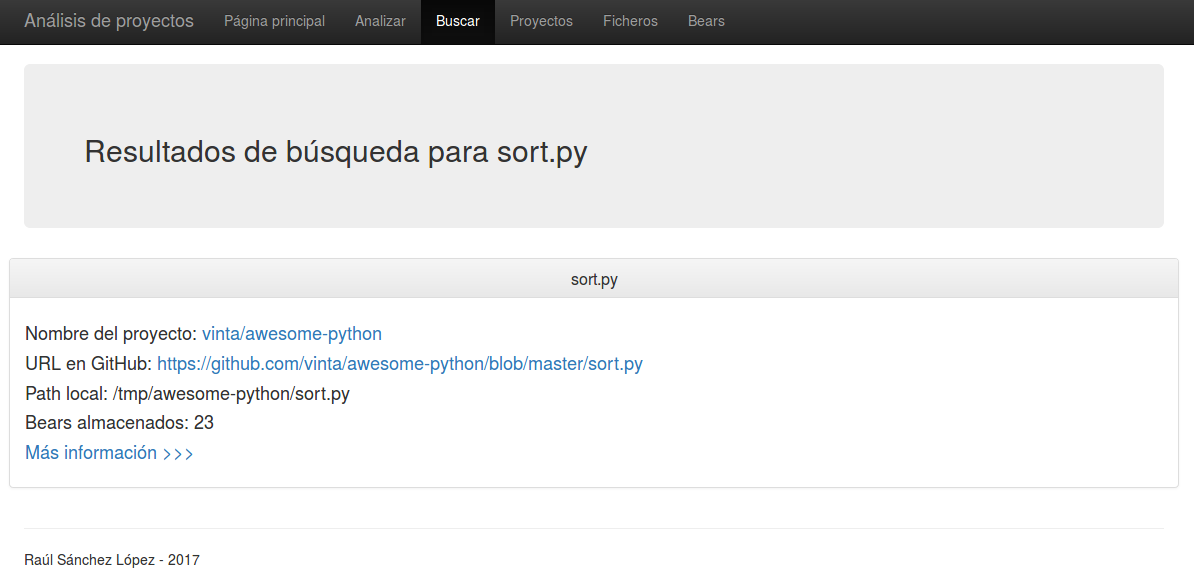
\includegraphics[width=12cm, keepaspectratio]{img/resultadoBuscar}
  \caption{Ejemplo de búsqueda por fichero.}
  \label{fig:resultadoBuscar}
\end{figure}

Si queremos ver un resumen de todos los proyecto, ficheros y bears almacenados, habrá que dirigirse al apartado correspondiente de la web. Los proyectos están ordenados de mayor a menor porcentaje de ficheros afectados por algún bear, los ficheros aparecen ordenados por cantidad de bears encontrados, sin tener en cuenta de que tipo son, y en el caso de los bears, aparecen ordenados los bears encontrados por tipo.

\begin{figure}[H]
  \centering
  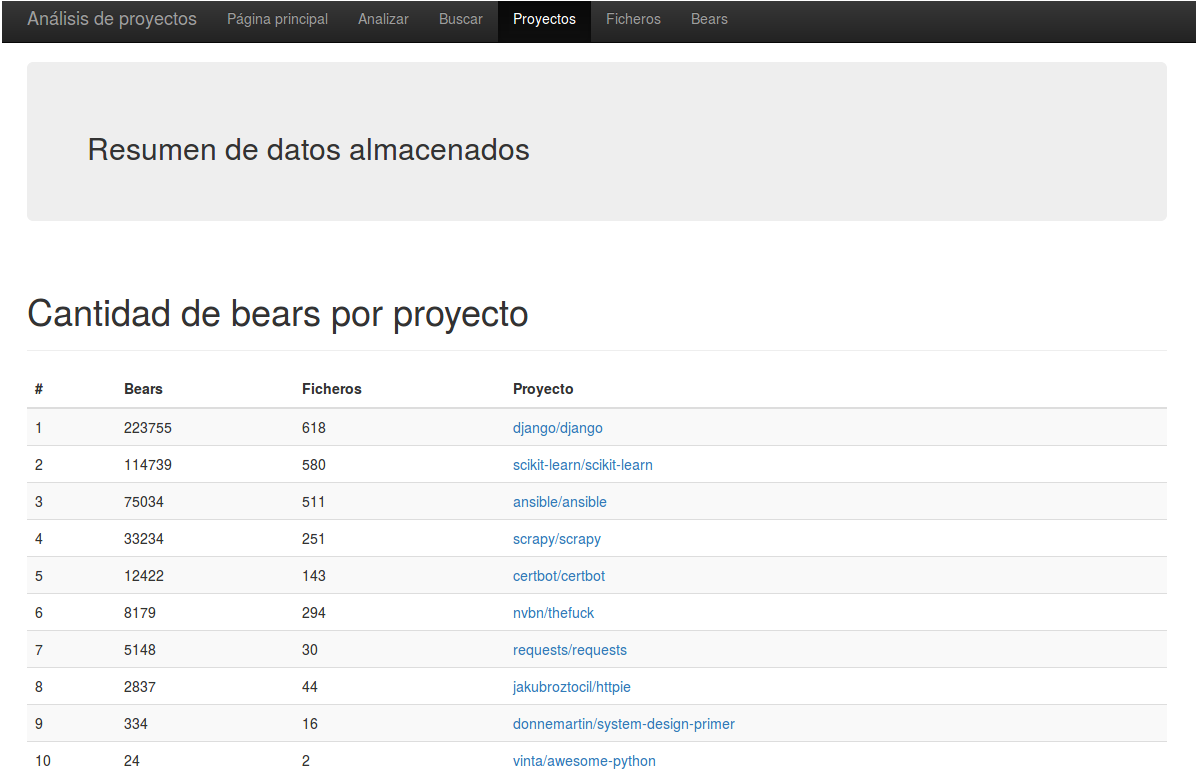
\includegraphics[width=15cm, keepaspectratio]{img/resumenProyectos}
  \caption{Página de resumen de proyectos almacenados ordenados por porcentaje de ficheros afectados.}
  \label{fig:resumenProyectos}
\end{figure}

\begin{figure}[H]
  \centering
  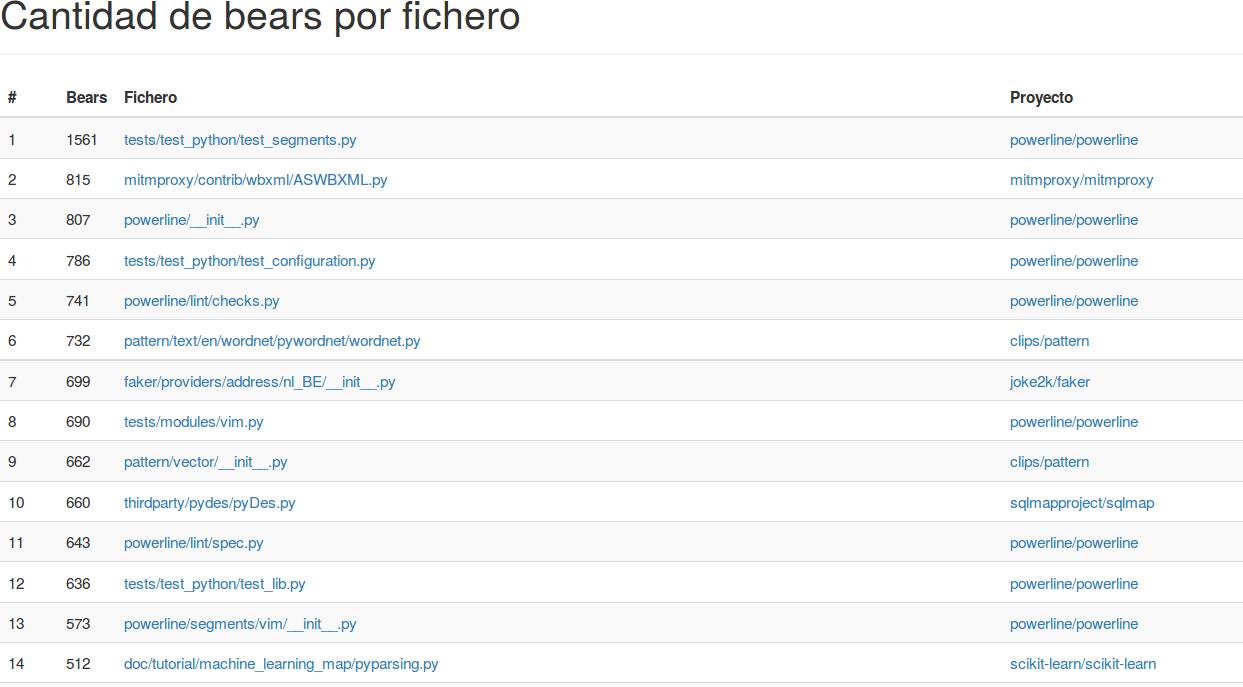
\includegraphics[width=15cm, keepaspectratio]{img/resumenFicheros}
  \caption{Información mostrada en la página de resumen de ficheros almacenados ordenados por cantidad de bears encontrados.}
  \label{fig:resumenFicheros}
\end{figure}

\begin{figure}[H]
  \centering
  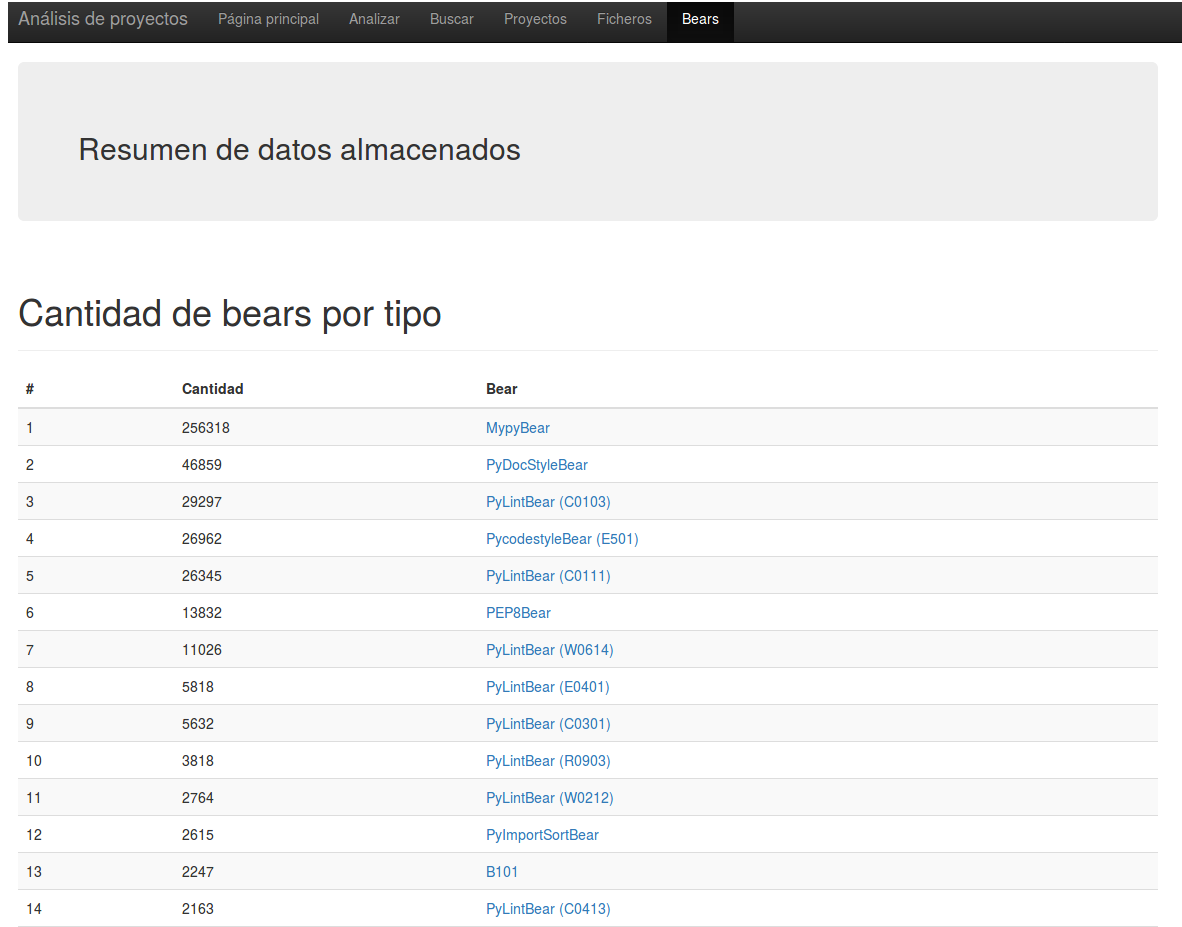
\includegraphics[width=11cm, keepaspectratio]{img/resumenBears}
  \caption{Información mostrada en la página de resumen de tipos bears almacenados.}
  \label{fig:resumenBears}
\end{figure}

Finalmente, tenemos las páginas de información de cada proyecto, fichero y bears. En ellas se muestra toda la información almacenada en la base de datos. Cuando analizamos un proyecto, podemos consultar la página del proyecto y a partir de ahí navegar por los diferentes ficheros y consultar los bears que se han encontrado, los mensajes que lanza cada uno de ellos, etc...

La página de proyecto muestra una información parecida a la que nos encontramos en la página de inicio, pero además tiene información sobre los ficheros almacenados para ese proyecto concreto. Esa información se puede mostrar u ocultar pinchando en el enlace correspondiente.
\begin{figure}[H]
  \centering
  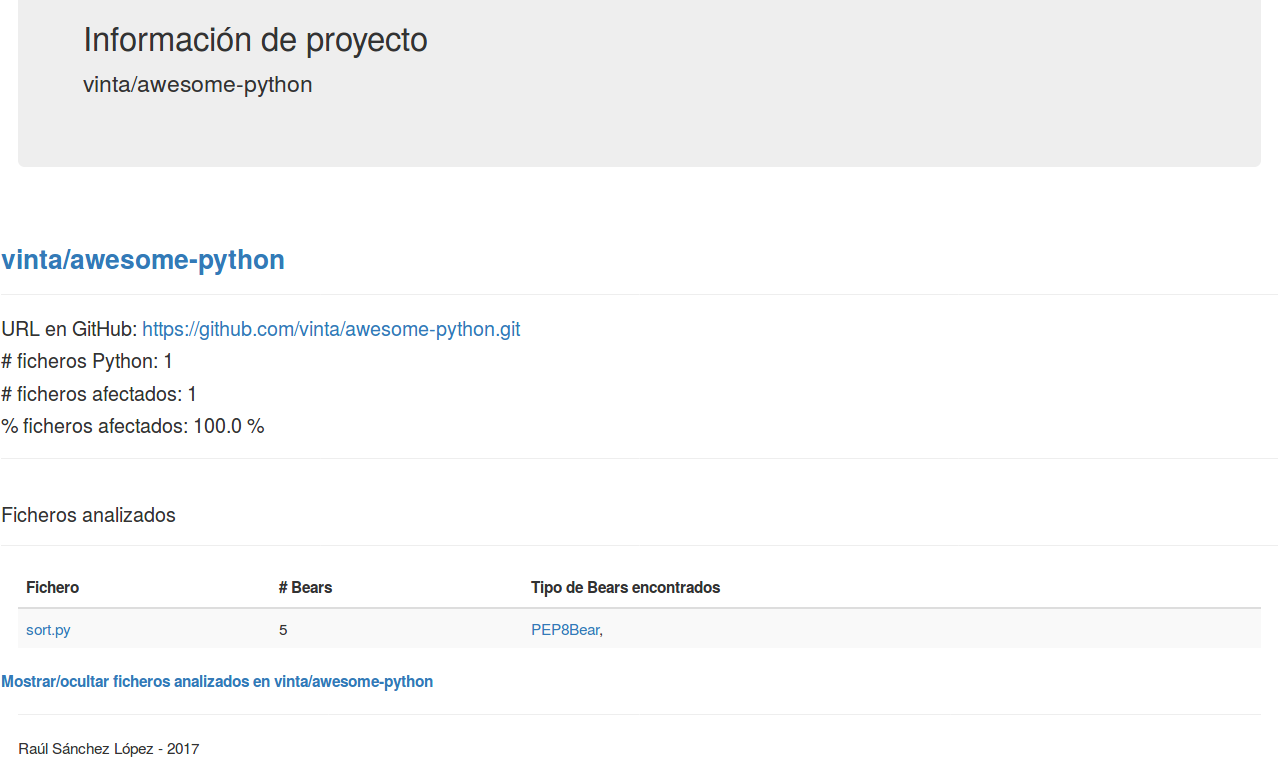
\includegraphics[width=16cm, keepaspectratio]{img/infoProyecto}
  \caption{Información mostrada en la página de información de proyecto.}
  \label{fig:infoProyecto}
\end{figure}

La página de información del fichero muestra los datos del fichero, además de una tabla con todos los bears encontrados. Esta tabla tiene los datos básicos, como son el tipo de bear, el mensaje lanzado, las líneas afectadas y el Id de cada uno de los bears.

La página de información del bear muestra todos los datos almacenados para cada bear. Esta es la página con mayor nivel de detalle tras hacer el análisis, puesto que en ella podemos ver el problema concreto que ha detectado la herramienta.

\begin{figure}[H]
  \centering
  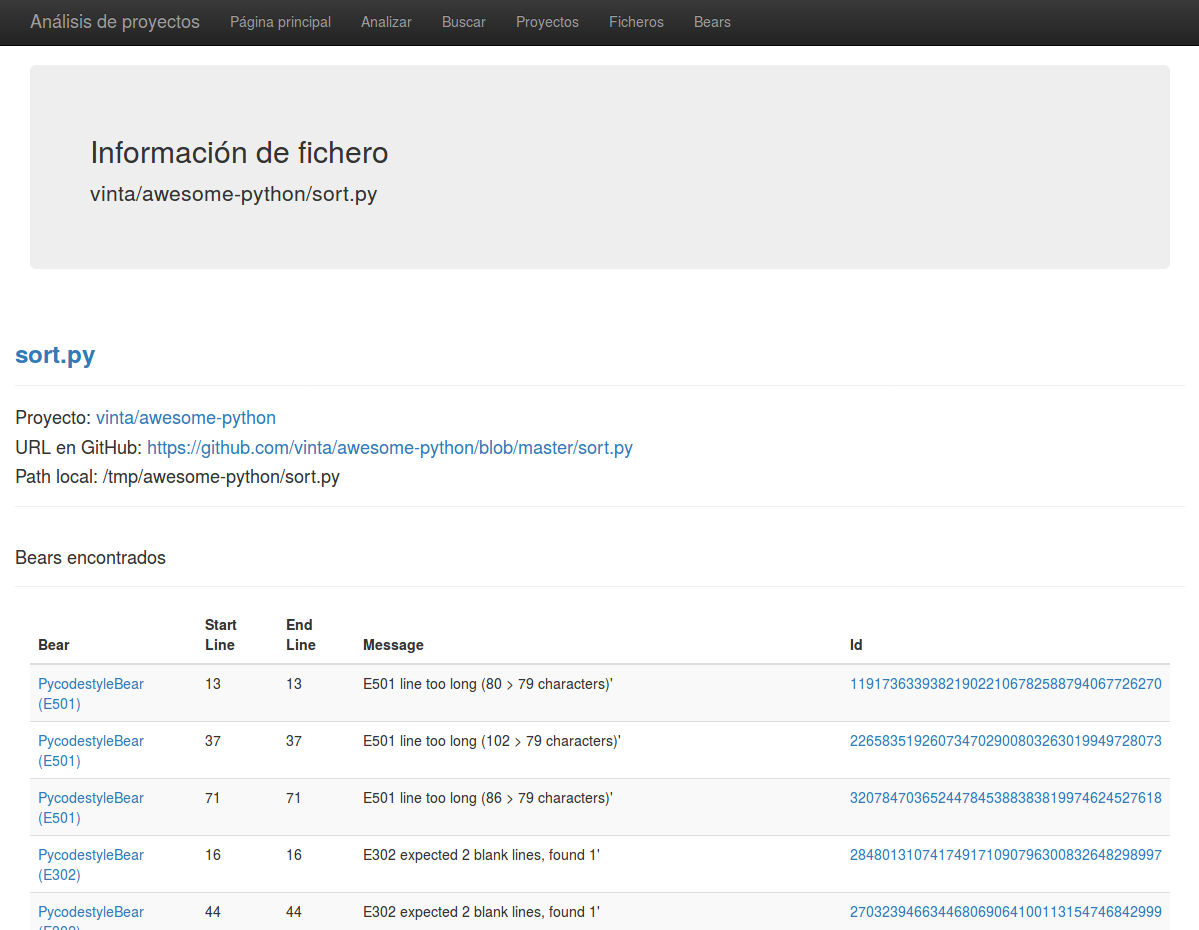
\includegraphics[width=16cm, keepaspectratio]{img/infoFichero}
  \caption{Información mostrada en la página de información de fichero.}
  \label{fig:infoFichero}
\end{figure}

\begin{figure}[H]
  \centering
  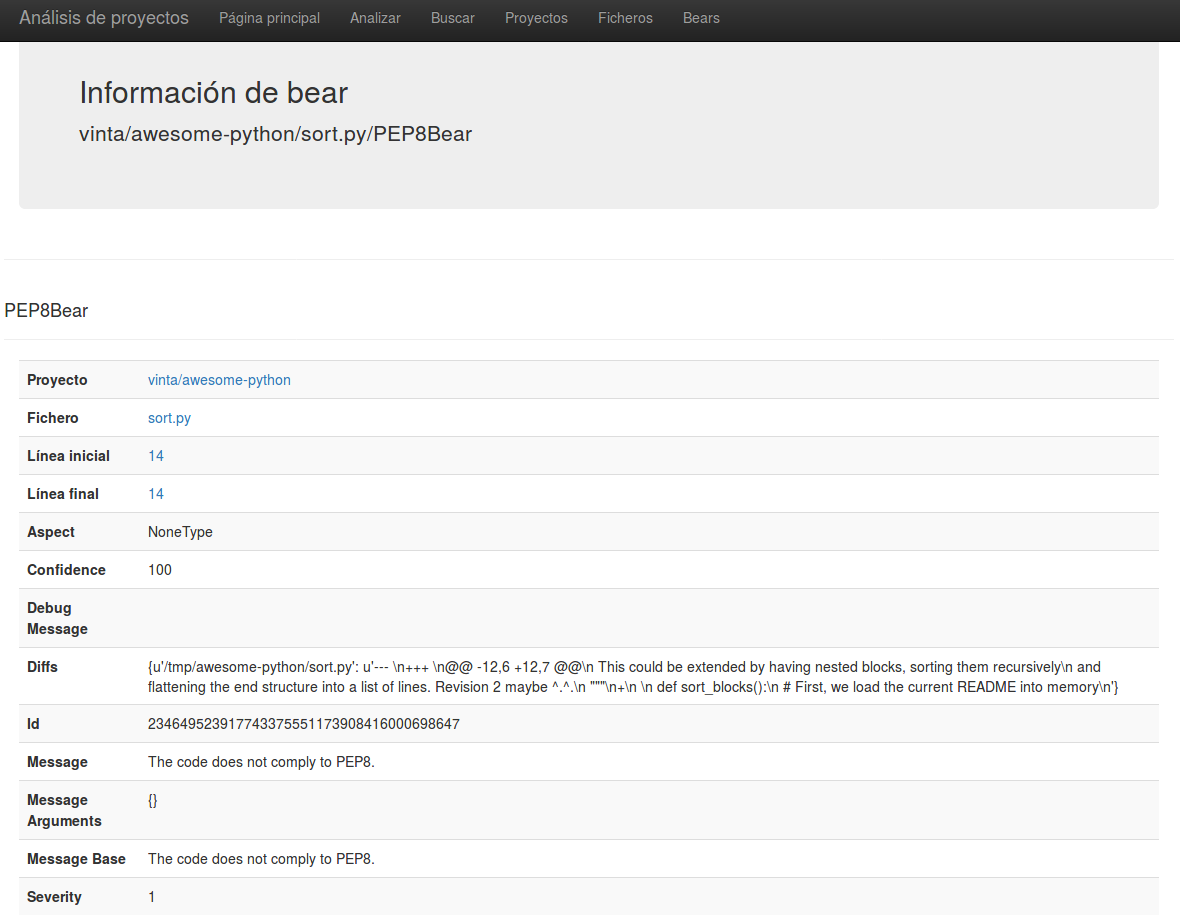
\includegraphics[width=16cm, keepaspectratio]{img/infoBear}
  \caption{Información mostrada en la página de información de bear.}
  \label{fig:infoBear}
\end{figure}

\section{Diseño e implementación de la base de datos} 
\label{sec:seccion14}
Es una base de datos relacional, en la que las distintas tablas están relacionadas entre sí por medio de algunos campos, tal y como se observaba en la figura~\ref{fig:EstructuraBBDD}.

\subsection{Project}
\label{sec:seccion14.1}
La tabla Project almacena la información de los proyectos. Para identificar un proyecto sólo es necesario tener su nombre y la URL en GitHub, aunque se añade la cantidad total de ficheros para su posterior uso.

\begin{itemize}
          \item Name: Nombre del proyecto analizado.
          \item URL: URL donde está alojado en proyecto en GitHub. Es la URL que hay que proporcionar a la aplicación para analizar proyectos.
          \item TotalFiles: Cantidad total de ficheros Python que forman el proyecto.
\end{itemize}

\subsection{File}
\label{sec:seccion14.2}
La tabla File almacena la información de los ficheros analizados en cada proyecto.

\begin{itemize}
          \item Name: Nombre del fichero.
          \item URL: URL donde se aloja el fichero en GitHub.
          \item ProjectName: Proyecto al que pertenece el fichero analizado.
          \item FilePath: Path local del fichero. Podemos definir donde se descargán dentro del fichero `settings' de Django.
\end{itemize}

\subsection{Bear}
\label{sec:seccion14.3}
Para la creación de la tabla Bear que contiene la información de los bears encontrados se han utilizado los datos de salida del análisis de Coala. Esta información aparece ordenada en el fichero JSON que se procesa durante el análisis.

\begin{itemize}
          \item Bear: Nombre del bear que ha detectado el problema. Algunos bears son herramientas que analizan muchos aspectos diferentes, por lo que este nombre puede ir seguido del código interno de esos bears o directamente puede tener el código como nombre.
          \item ProjectName: Proyecto al que pertenece la incidencia encontrada por el bear.
          \item FileName: Fichero en el que se ha encontrado la incidencia.
          \item StartLine: Línea donde comienza la incidencia detectada por el bear. En caso de que la incidencia encontrada no se refiera a ninguna línea en concreto por tratarse de un problema en el propio fichero, como por ejemplo convenciones de nombrado, será 0. También será 0 cuando la incidencia no se refiera a un fichero en concreto, sino a a un problema general del proyecto analizado.
          \item StartLineURL: URL de GitHub que lleva a la línea donde comienza la incidencia. Será `None' en caso de que la línea sea 0 por los supuestos anteriores.
          \item EndLine: Línea donde termina la incidencia detectada por el bear. También será 0 en los supuestos descritos para `StartLine'.
          \item EndLineURL: URL de GitHub que lleva a la línea donde termina la incidencia. También será `None' en los supuestos descritos para `StartLine'.
          \item Aspect: Hoja de la clase `Aspect' a la que pertenece este resultado. Para los términos de este trabajo se incluyó por formar parte de la salida de Coala, pero en principio no aporta mas información.
          \item Confidence: Número entre 0 y 100 que describe la probabilidad de que la incidencia sea un problema real.
          \item DebugMsg: Mensaje que puede ayudar al usuario a averiguar por qué se obtuvo el resultado.
          \item Diffs: Diccionario con nombres de fichero asociados a la secuencia de código que provocó la incidencia. No todos los bear ofrecen esta información, por lo que en muchas ocasiones puede aparecer vacío.
          \item BearId: Número de identificación del bear.
          \item Message: Mensaje que lanza el bear informando del problema encontrado.
          \item MessageArguments: Argumentos extra del mensaje. Para los términos de este trabajo se incluyó por formar parte de la salida de Coala, pero en principio no aporta mas información.
          \item MessageBase: Texto base del mensaje. Para los términos de este trabajo se incluyó por formar parte de la salida de Coala, pero en principio no aporta mas información.
          \item Severity: Severidad del mensaje.
\end{itemize}

%%%%%%%%%%%%%%%%%%%%%%%%%%%%%%%%%%%%%%%%%%%%%%%%%%%%%%%%%%%%%%%%%%%%%%%%%%%%%%%%
%%%%%%%%%%%%%%%%%%%%%%%%%%%%%%%%%%%%%%%%%%%%%%%%%%%%%%%%%%%%%%%%%%%%%%%%%%%%%%%%
% RESULTADOS %
%%%%%%%%%%%%%%%%%%%%%%%%%%%%%%%%%%%%%%%%%%%%%%%%%%%%%%%%%%%%%%%%%%%%%%%%%%%%%%%%

\cleardoublepage
\chapter{Resultados}
Para comprender la utilidad de la aplicación, vamos a analizar una lista de 50 proyectos\footnote{Dentro de los 52 con mas estrellas sólo se han excluido 2 por tamaño.} dentro de aquellos que cuentan con más estrellas en GitHub. Para ello, vamos a utilizar un fichero de configuración en el que incluiremos, en lugar de todo el listado disponible para Python, una selección de bears para centrarnos solo en algunos aspectos y evitando aquellos bears que hacen un análisis completo por si mismos. De este modo se pretende clasificar los resultados por los datos concretos que analiza cada uno de estos bears.

\section{Fichero de configuración}
\label{sec:_coafile}
Para la prueba utilizaré el siguiente `.coafile':

{\footnotesize
\begin{verbatim}
    [Default]
    bears = FilenameBear,PEP8Bear,PyCommentedCodeBear,VultureBear,
    SpaceConsistencyBear
    files = *.py
    use_spaces = True
\end{verbatim}
}
`FileNameBear' comprobará que el nombre de los ficheros sigue la convención `snake', `PEP8Bear' comprobará que se sigue la guía de estilo descrita en PEP8, `PyCommentedCodeBear' buscará código fuente comentado, `VultureBear' buscará clases, funciones y variables que no son utilizadas y finalmente `SpaceConsistencyBear' comprobará el espaciado. Todos los bears utilizaran la configuración por defecto y en el caso de `SpaceConsistencyBear' habilitamos la opción que obliga al uso de espacios en lugar de tabulaciones.

\section{Análisis de datos recogidos}
\label{sec:_datarec}
Tras finalizar el análisis, consultamos el resumen de Bears. El tipo de bear que se ha dectectado un mayor número de veces es el `PEP8Bear', de donde se puede concluir que, dentro de este escenario, el principal problema de los proyectos con mejor valoración tiene que ver con el estilo, aunque este bear no especifica exactamente en su mensaje el error encontrado.

\begin{figure}[H]
  \centering
  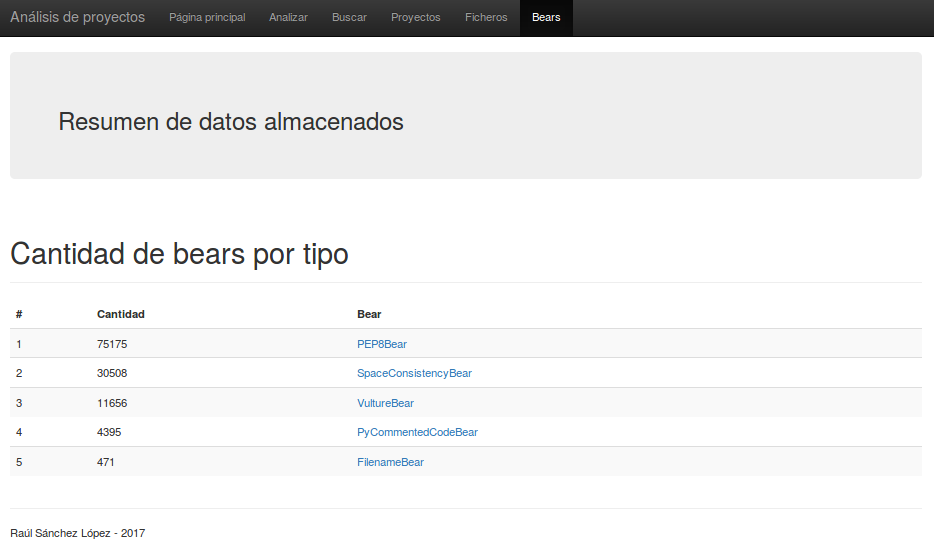
\includegraphics[width=15cm, keepaspectratio]{img/resultadosBear}
  \caption{Página de resumen de bears recogidos.}
  \label{fig:resultadosBear}
\end{figure}

El siguiente bear de la lista es `SpaceConsistencyBear', por lo que muchos de estos proyectos cuentan con problemas de espaciado y utilizan tabulaciones en lugar de espacios. El tercer elemento de la lista es `VultureBear', seguido de `PyCommentedCode' y terminando por `FileNameBear' en un número bastante inferior.

De todo lo anterior se deduce que incluso los proyectos mejor valorados tienen problemas de estilo, pero sin embargo es poco frecuente que sus ficheros no sigan la convención `snake'.

Ahora vamos a hacer una comparación entre proyectos. Uno de los datos que podemos visualizar con la aplicación es el porcentaje de ficheros que cuentan con, al menos, un bear detectado, es decir, un problema a priori:

\begin{figure}[H]
  \centering
  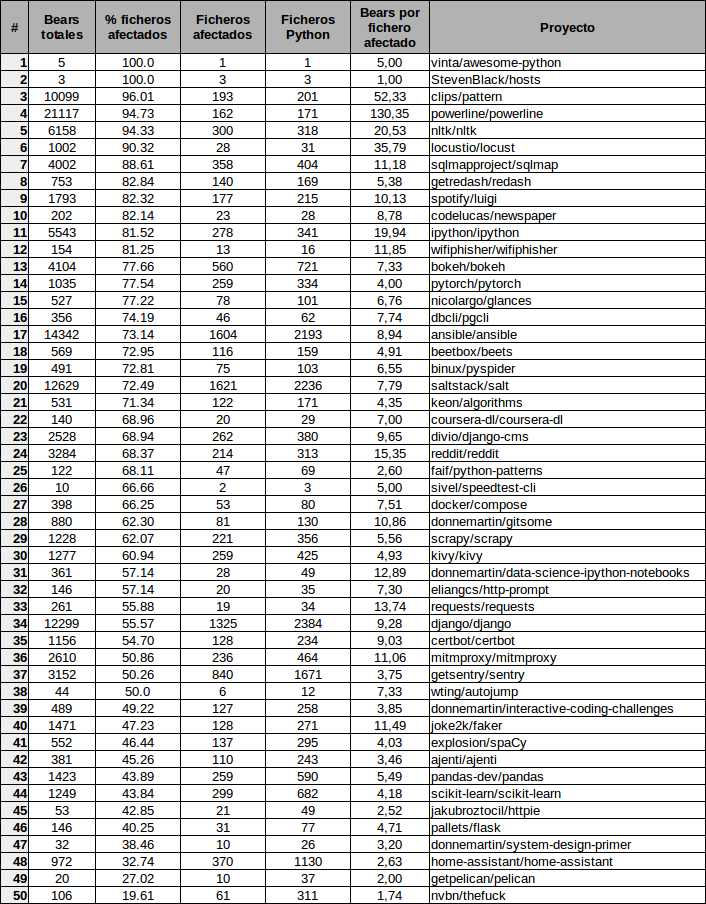
\includegraphics[width=15cm, keepaspectratio]{img/anexoTabla}
  \caption{Lista de proyectos analizados.}
  \label{fig:anexoTabla}
\end{figure}

En la tabla anterior se ha añadido una columna con información que no procede de la aplicación, obtenida de hacer una división entre la cantidad de bears encontrados y la cantidad de ficheros afectados: `Bears por fichero afectado'.

Dentro de este escenario, el proyecto con un menor porcentaje de ficheros Python afectados por algún bear es `thefuck', cuyo creador es `nvbn'. ¿Esto hace de `thefuck' el proyecto con menos `errores' del listado? La respuesta es que depende. Es el que menos ficheros tiene afectados por algún bear en términos absolutos, y a su vez uno de los mejores en cantidad de bears por fichero afectado. Además, el fichero que cuenta con más errores tiene 8, relacionados con el estilo, código en desuso y el uso de espacios.

\begin{figure}[H]
  \centering
  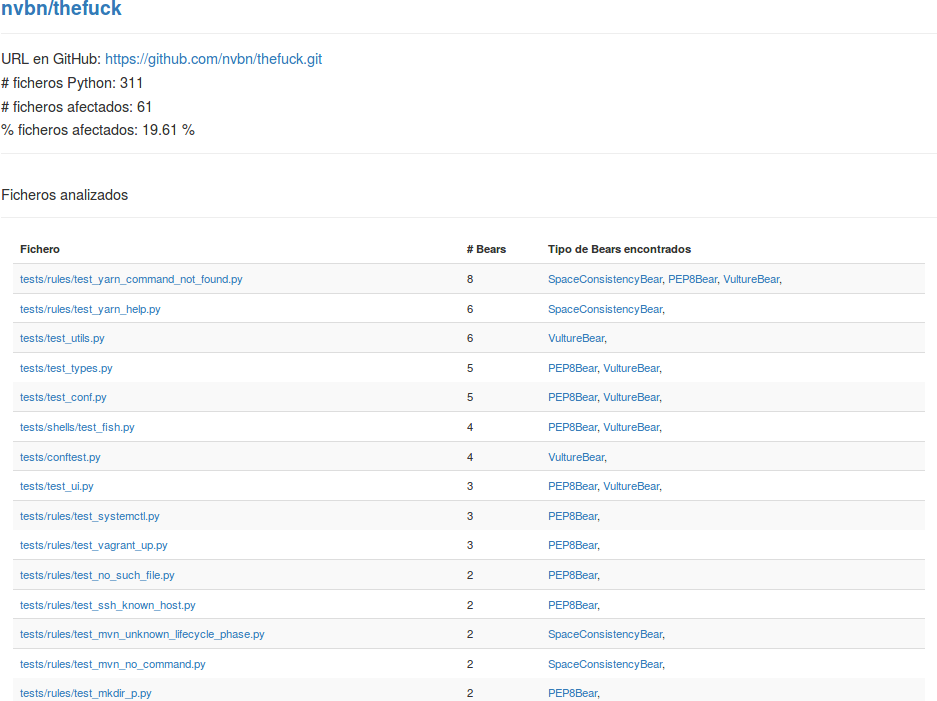
\includegraphics[width=16cm, keepaspectratio]{img/theFuckInfo}
  \caption{Extracto de lista de ficheros afectados en `thefuck'.}
  \label{fig:theFuckInfo}
\end{figure}

Por ejemplo el proyecto `hosts' de `StevenBlack' tiene errores en todos sus ficheros Python, pero son errores sobre la convención de nombrado de los ficheros (`FilenameBear'), en total es en el que menos bears se han encontrado, pero se trata de un proyecto pequeño en cuanto al número de ficheros totales en comparación con el resto de proyectos de la lista. Además, estos problemas son fácilmente reparables si queremos utilizar la convención de nombrado tipo `snake', ya que basta con renombrarlos.

\begin{figure}[H]
  \centering
  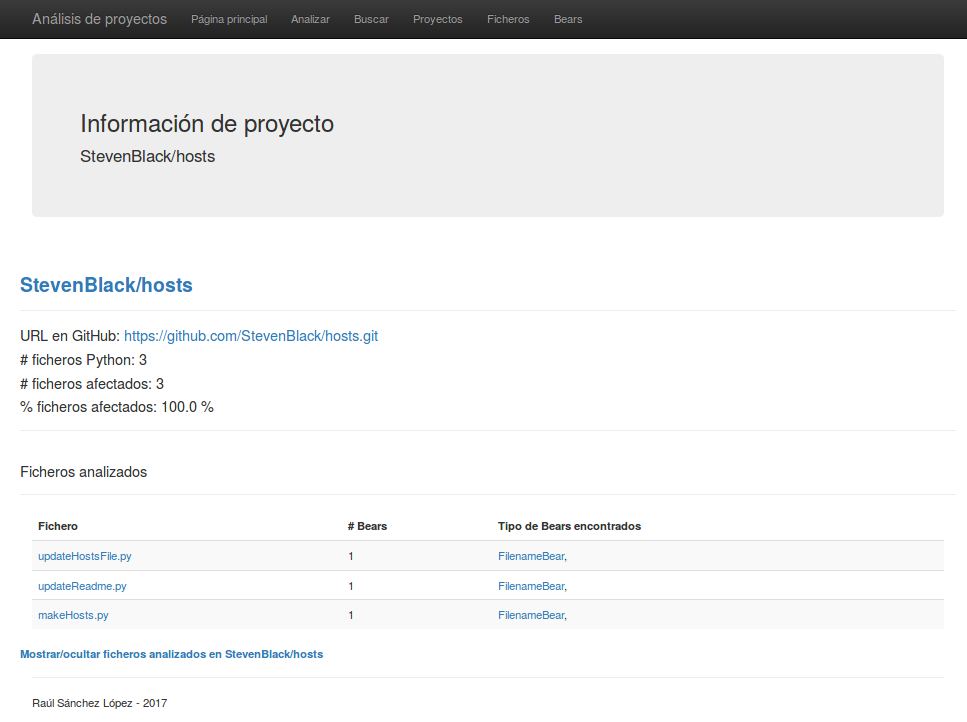
\includegraphics[width=15cm, keepaspectratio]{img/proyectoHosts}
  \caption{Información mostrada en la página del proyecto `hosts'.}
  \label{fig:proyectoHosts}
\end{figure}

Si tenemos en cuenta el número total de ficheros Python de cada proyecto, sin duda `thefuck' destaca sobre el resto.

Para recabar más información sobre el proyecto `thefuck', habría que inspeccionar los ficheros almacenados. Por ejemplo, el fichero `test\_yarn\_command\_not\_found.py', que es el que mayor número de bears acumula en este proyecto.

Como se observa en la figura~\ref{fig:ficheroTheFuck}, la mayor parte de errores vienen de la inclusión de espacios al final o al inicio de una sentencia. 

\begin{figure}[H]
  \centering
  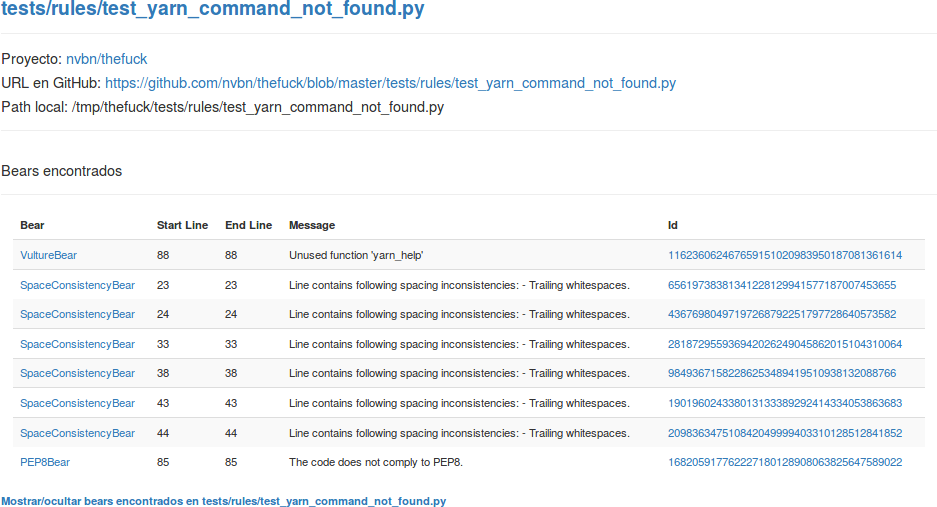
\includegraphics[width=15cm, keepaspectratio]{img/ficheroTheFuck}
  \caption{Detalle de bears encontrados en un fichero de `thefuck'.}
  \label{fig:ficheroTheFuck}
\end{figure}

Podemos ver en más detalle uno de los bears de la lista a través del enlace. Ahí se muestra toda la información que ha recopilado Coala.

\begin{figure}[H]
  \centering
  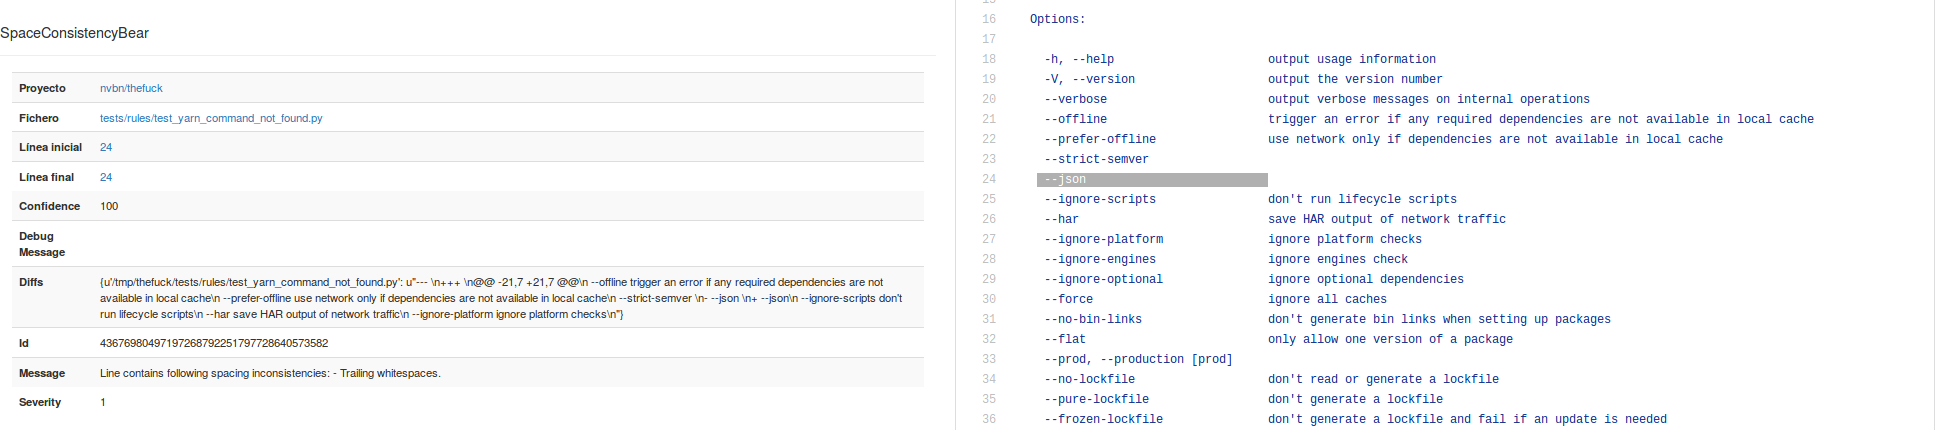
\includegraphics[width=17cm, keepaspectratio]{img/bearData}
  \caption{Detalle de uno de los bears encontrados por la aplicación.}
  \label{fig:bearData}
\end{figure}

Para ver exactamente donde se encuentra el fallo, podemos inspeccionar el fichero a través del enlace a la línea exacta desde la información de bear, en este caso la línea 24. Una vez abierto, comprobaremos que existe al menos un espacio en blanco a la derecha de `--json' que ha detectado el `SpaceConsistencyBear', ya que con la configuración utilizada para este análisis no permite estos espacios.

\begin{figure}[H]
  \centering
  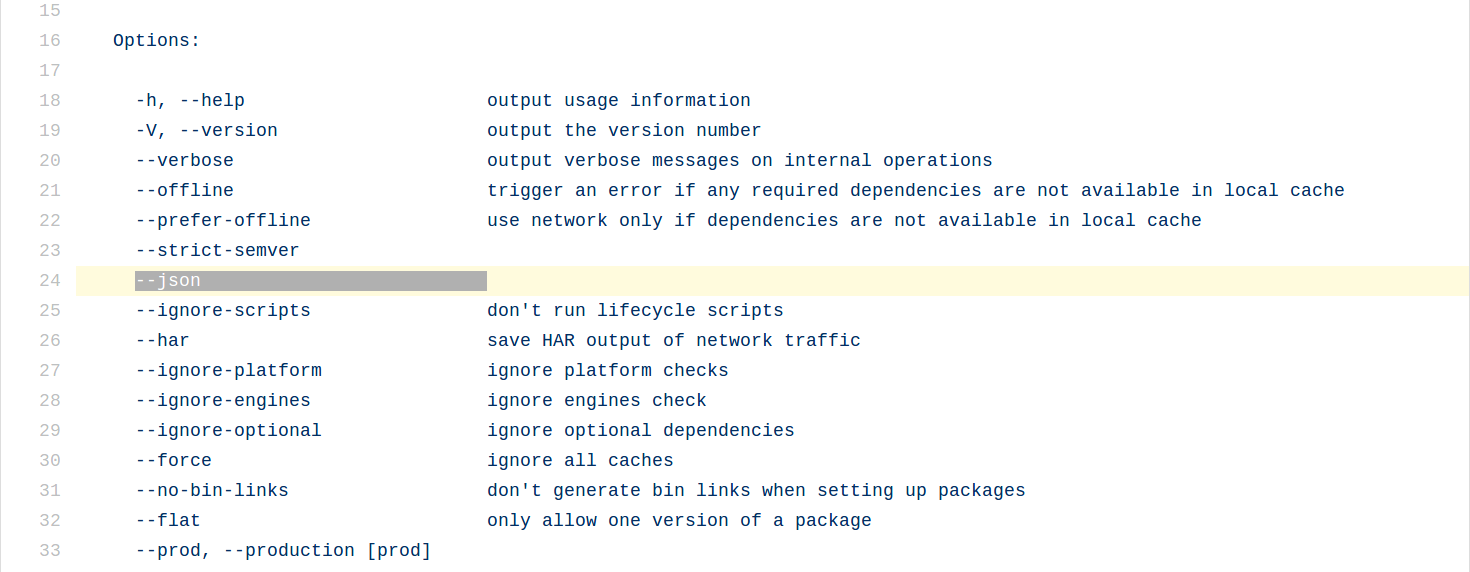
\includegraphics[width=17cm, keepaspectratio]{img/bearDataGitHub}
  \caption{Detalle de uno de los bears encontrados en GitHub.}
  \label{fig:bearDataGitHub}
\end{figure}

De este modo, la aplicación nos ayuda a detectar errores y corregir el código en caso de ser necesario. 

Uno de los principales ejemplos de uso sería analizar un proyecto propio de GitHub y a partir de los resultados del análisis, evaluar los errores que ha detectado la aplicación y corregir aquellos que consideremos necesarios para mejorar el funcionamiento del proyecto o ajustarnos a las normas de estilo establecidas.

%%%%%%%%%%%%%%%%%%%%%%%%%%%%%%%%%%%%%%%%%%%%%%%%%%%%%%%%%%%%%%%%%%%%%%%%%%%%%%%%
%%%%%%%%%%%%%%%%%%%%%%%%%%%%%%%%%%%%%%%%%%%%%%%%%%%%%%%%%%%%%%%%%%%%%%%%%%%%%%%%
% CONCLUSIONES %
%%%%%%%%%%%%%%%%%%%%%%%%%%%%%%%%%%%%%%%%%%%%%%%%%%%%%%%%%%%%%%%%%%%%%%%%%%%%%%%%

\cleardoublepage
\chapter{Conclusiones}
\label{chap:conclusiones}


\section{Consecución de objetivos}
\label{sec:consecucion-objetivos}

Esta sección es la sección espejo del capítulo de objetivos, donde se revisará si se han alcanzado los objetivos marcados al inicio de este trabajo. Para hacer esta valoración iré de los objetivos más específicos hasta el objetivo general.

Para poder desarrollar la aplicación el primer paso era aprender a utilizar Coala y estudiar cada uno de los bears que podemos utilizar. Para ello estudié el funcionamiento de la aplicación y los bears descritos en el Capítulo 2. Cada uno de estos bears tiene una funcionalidad distinta y consta de diferentes opciones de configuración.

Una vez estudiado el funcionamiento de Coala, era necesario mapear la salida del fichero JSON para poder almacenar la información correctamente. Tras esto, la aplicación era capaz de mostrar todos los campos contenidos en ese fichero sin ningún tipo de problema, tratando los datos de forma que se acoplaran a los resultados obtenidos en cada análisis, como por ejemplo, contemplando casos en los que no existe una línea afectada por tratarse de un bear que se refiere a todo el fichero o la configuración del proyecto en su totalidad.

Antes de poner en marcha la aplicación en Django, había que probar que todo encajaba correctamente. La primera versión del programa servía para testear que las asunciones hechas anteriormente eran las correctas y el análisis arrojaba los resultados esperados. Tras una serie de pruebas, la herramienta era capaz de analizar un listado de proyectos procedentes de un fichero.

El siguiente paso era trasladar aquella lógica a Django, para presentar los resultados en forma de página web y almacenar la información en una base de datos. Django facilita mucho la tarea de lidiar con bases de datos debido a su simplicidad a la hora de almacenar y consultar la información.

Finalmente quedaba crear todos los `templates' necesarios para presentar la información al usuario. Justo en este punto se empieza a optimizar el funcionamiento de la aplicación y se añaden nuevas funcionalidades como el resumen de datos, la búsqueda, análisis de ficheros a partir de una URL, eliminación de proyectos almacenados (aunque sea una función que no se presente al usuario por estar pensada para el administrador), ordenar la información o incluir el porcentaje de ficheros afectados en el proyecto.

El objetivo principal de este trabajo era el desarrollo de una aplicación web que sirviera para analizar código fuente Python. Revisando todo lo anterior llegamos a la conclusión de que el objetivo principal se ha cumplido.

\section{Aplicación de lo aprendido}
\label{sec:aplicacion}
En la elaboración de este trabajo se han utilizado numerosas tecnologías. Algunas de ellas eran totalmente desconocidas para mí, pero otras formaban parte del temario de asignaturas cursadas a lo largo de la carrera:

\begin{enumerate}
  \item Conocimiento adquiridos en SAT: es la asignatura en la que aprendí la mayor parte de de los conocimiento aplicados en este proyecto. En ella adquirí conocimientos de Python, Django, HTML, CSS,... por lo que está estrechamente relacionada con este proyecto.
  \item Arquitectura cliente-servidor: vista en más de una asignatura, llegando a presentar numerosas prácticas con este modelo aunque no solo en Python, también utilizando otros lenguajes como Java.
\end{enumerate}


\section{Lecciones aprendidas}
\label{sec:lecciones_aprendidas}
Para la realización de este proyecto he aprendido a utilizar herramientas y tecnologías que desconocía o que no había usado hasta este momento:

\begin{enumerate}
  \item Coala: no tenía conocimiento de la existencia de esta herramienta hasta que mi tutor me habló de ello. Es de gran utilidad para el análisis de código gracias a que a partir de una sola herramienta y gracias a sus numerosos bears podemos hacer análisis de todo tipo.
  \item Git/GitHub: es otra de las claves de este proyecto. Me ha servido tanto para encontrar los proyectos que he analizado como para alojar el proyecto en sí mismo. Facilita mucho el control de versiones y la posibilidad de colaborar en proyectos o que otros desarrolladores colaboren en tu proyecto.
  \item BootStrap: para mí ha sido un gran descubrimiento. Es de enorme utilidad a la hora de diseñar páginas web. Ha sido de mucha ayuda a la hora de mejorar el aspecto de las diferentes vistas de la aplicación.
  \item JSON: conocía la tecnología, pero no lo había utilizado tanto hasta la elaboración de este trabajo. Me ha facilitado mucho el tratamiento de los datos procedentes de los análisis.
\end{enumerate}


\section{Trabajos futuros}
\label{sec:trabajos_futuros}
Ningún software se termina, todas las aplicaciones necesitan nuevas funcionalidades y requieren de constantes actualizaciones. Es proyecto no se escapa a este aspecto y, como todas, está abierto a mejoras.

Una de las funciones más interesantes sería la elaboración de una clasificación o ranking de `calidad' de los proyectos a partir de los datos recogidos. Aunque se analizan los ficheros y se da una idea a partir de los datos recogidos, se podría entrar más en detalle clasificando la gravedad de cada bear respecto al resto y no solo la cantidad. Dentro de este ámbito de la `calidad', se podrían hacer muchas clasificaciones diferentes y tener diferentes rankings dependiendo de factores concretos.

Otra funcionalidad extra podría apoyarse en la capacidad de algunos bears de reparar los problemas detectados, configurando los bears compatibles para solucionar estos problemas y hacer un pull request al creador del proyecto de forma automática.

%%%%%%%%%%%%%%%%%%%%%%%%%%%%%%%%%%%%%%%%%%%%%%%%%%%%%%%%%%%%%%%%%%%%%%%%%%%%%%%%
%%%%%%%%%%%%%%%%%%%%%%%%%%%%%%%%%%%%%%%%%%%%%%%%%%%%%%%%%%%%%%%%%%%%%%%%%%%%%%%%
% APÉNDICE(S) %
%%%%%%%%%%%%%%%%%%%%%%%%%%%%%%%%%%%%%%%%%%%%%%%%%%%%%%%%%%%%%%%%%%%%%%%%%%%%%%%%

\cleardoublepage
\appendix
\chapter{Manual de usuario}
\label{app:manual}

\section{Instalación de Coala}
\label{app:inst_coala}
Antes de poder utilizar la aplicación es necesario instalar Coala en el equipo. Para ello hay que ejecutar en una terminal el siguiente comando para su instalación simple:
{\footnotesize
\begin{verbatim}
    $ pip3 install coala-bears
\end{verbatim}
}

Sin embargo, si se va a utilizar un entorno virtual:
{\footnotesize
\begin{verbatim}
    $ pip3 install virtualenv
    $ virtualenv venv        # On Linux
    $ venv\scripts\activate  # On Windows
\end{verbatim}
}

\section{Instalación de Django}
\label{app:inst_Django}
Para poder utilizar la aplicación es necesario tener instalado Django. Para ello hay que ejecutar:
{\footnotesize
\begin{verbatim}
    $ pip install django
\end{verbatim}
}

Para lanzar el servidor hay que abrir una terminal en la ruta en la que se encuentra el proyecto y ejecutar:
{\footnotesize
\begin{verbatim}
    $ python manage.py runserver
\end{verbatim}
}
Esto lanzará el servidor con la configuración por defecto, que es la utilizada en este proyecto.

\section{Uso del analizador}
\label{app:analyzer}
Se puede descargar o clonar el proyecto desde su página de GitHub:
{\footnotesize
\begin{verbatim}
   https://github.com/rsanlo/prAnalysis
\end{verbatim}
}

Antes de ejecutar el servidor, hay que configurar las rutas por defecto en el fichero de Django dentro de `/prAnalysis/settings.py'. Los datos a editar son `workspace', que es el lugar donde descargará los proyectos para analizarlos y donde buscará el fichero de configuración `.coafile', y `jsonFile', que es donde almacenará y consultará el fichero JSON.
{\footnotesize
\begin{verbatim}
    # GLOBAL CONSTANTS
    CONSTANTS = {
    `workspace': `/tmp',
    `jsonFile': `/tmp/coala_analysis.json',
\end{verbatim}
}
Una vez hecho esto, hay que situar el fichero `.coafile' en la ruta definida. Su estructura debe ser como sigue:
{\footnotesize
\begin{verbatim}
    [Default]
    bears = Bear1, Bear2, Bear3,...
    opcionA = valorA
    opcionB = valorB
    .
    .
    .
\end{verbatim}
}

En `bears' añadimos los bears que queremos utilizar y debajo las opciones que vayamos a configurar para cada uno de ellos.

El cliente accederá a la página principal a través de la siguiente URL:
{\footnotesize
\begin{verbatim}
   http://localhost:8000/analyzer
\end{verbatim}
}


%%%%%%%%%%%%%%%%%%%%%%%%%%%%%%%%%%%%%%%%%%%%%%%%%%%%%%%%%%%%%%%%%%%%%%%%%%%%%%%%
%%%%%%%%%%%%%%%%%%%%%%%%%%%%%%%%%%%%%%%%%%%%%%%%%%%%%%%%%%%%%%%%%%%%%%%%%%%%%%%%
% BIBLIOGRAFIA %
%%%%%%%%%%%%%%%%%%%%%%%%%%%%%%%%%%%%%%%%%%%%%%%%%%%%%%%%%%%%%%%%%%%%%%%%%%%%%%%%

\cleardoublepage

% Las siguientes dos instrucciones es todo lo que necesitas
% para incluir las citas en la memoria
\bibliographystyle{abbrv}
\bibliography{memoria}  % memoria.bib es el nombre del fichero que contiene
% las referencias bibliográficas. Abre ese fichero y mira el formato que tiene,
% que se conoce como BibTeX. Hay muchos sitios que exportan referencias en
% formato BibTeX. Prueba a buscar en http://scholar.google.com por referencias
% y verás que lo puedes hacer de manera sencilla.
% Más información: 
% http://texblog.org/2014/04/22/using-google-scholar-to-download-bibtex-citations/

\end{document}
\grid
\grid
\grid
\grid
